\documentclass[1p]{elsarticle_modified}
%\bibliographystyle{elsarticle-num}

%\usepackage[colorlinks]{hyperref}
%\usepackage{abbrmath_seonhwa} %\Abb, \Ascr, \Acal ,\Abf, \Afrak
\usepackage{amsfonts}
\usepackage{amssymb}
\usepackage{amsmath}
\usepackage{amsthm}
\usepackage{scalefnt}
\usepackage{amsbsy}
\usepackage{kotex}
\usepackage{caption}
\usepackage{subfig}
\usepackage{color}
\usepackage{graphicx}
\usepackage{xcolor} %% white, black, red, green, blue, cyan, magenta, yellow
\usepackage{float}
\usepackage{setspace}
\usepackage{hyperref}

\usepackage{tikz}
\usetikzlibrary{arrows}

\usepackage{multirow}
\usepackage{array} % fixed length table
\usepackage{hhline}

%%%%%%%%%%%%%%%%%%%%%
\makeatletter
\renewcommand*\env@matrix[1][\arraystretch]{%
	\edef\arraystretch{#1}%
	\hskip -\arraycolsep
	\let\@ifnextchar\new@ifnextchar
	\array{*\c@MaxMatrixCols c}}
\makeatother %https://tex.stackexchange.com/questions/14071/how-can-i-increase-the-line-spacing-in-a-matrix
%%%%%%%%%%%%%%%

\usepackage[normalem]{ulem}

\newcommand{\msout}[1]{\ifmmode\text{\sout{\ensuremath{#1}}}\else\sout{#1}\fi}
%SOURCE: \msout is \stkout macro in https://tex.stackexchange.com/questions/20609/strikeout-in-math-mode

\newcommand{\cancel}[1]{
	\ifmmode
	{\color{red}\msout{#1}}
	\else
	{\color{red}\sout{#1}}
	\fi
}

\newcommand{\add}[1]{
	{\color{blue}\uwave{#1}}
}

\newcommand{\replace}[2]{
	\ifmmode
	{\color{red}\msout{#1}}{\color{blue}\uwave{#2}}
	\else
	{\color{red}\sout{#1}}{\color{blue}\uwave{#2}}
	\fi
}

\newcommand{\Sol}{\mathcal{S}} %segment
\newcommand{\D}{D} %diagram
\newcommand{\A}{\mathcal{A}} %arc


%%%%%%%%%%%%%%%%%%%%%%%%%%%%%5 test

\def\sl{\operatorname{\textup{SL}}(2,\Cbb)}
\def\psl{\operatorname{\textup{PSL}}(2,\Cbb)}
\def\quan{\mkern 1mu \triangleright \mkern 1mu}

\theoremstyle{definition}
\newtheorem{thm}{Theorem}[section]
\newtheorem{prop}[thm]{Proposition}
\newtheorem{lem}[thm]{Lemma}
\newtheorem{ques}[thm]{Question}
\newtheorem{cor}[thm]{Corollary}
\newtheorem{defn}[thm]{Definition}
\newtheorem{exam}[thm]{Example}
\newtheorem{rmk}[thm]{Remark}
\newtheorem{alg}[thm]{Algorithm}

\newcommand{\I}{\sqrt{-1}}
\begin{document}

%\begin{frontmatter}
%
%\title{Boundary parabolic representations of knots up to 8 crossings}
%
%%% Group authors per affiliation:
%\author{Yunhi Cho} 
%\address{Department of Mathematics, University of Seoul, Seoul, Korea}
%\ead{yhcho@uos.ac.kr}
%
%
%\author{Seonhwa Kim} %\fnref{s_kim}}
%\address{Center for Geometry and Physics, Institute for Basic Science, Pohang, 37673, Korea}
%\ead{ryeona17@ibs.re.kr}
%
%\author{Hyuk Kim}
%\address{Department of Mathematical Sciences, Seoul National University, Seoul 08826, Korea}
%\ead{hyukkim@snu.ac.kr}
%
%\author{Seokbeom Yoon}
%\address{Department of Mathematical Sciences, Seoul National University, Seoul, 08826,  Korea}
%\ead{sbyoon15@snu.ac.kr}
%
%\begin{abstract}
%We find all boundary parabolic representation of knots up to 8 crossings.
%
%\end{abstract}
%\begin{keyword}
%    \MSC[2010] 57M25 
%\end{keyword}
%
%\end{frontmatter}

%\linenumbers
%\tableofcontents
%
\newcommand\colored[1]{\textcolor{white}{\rule[-0.35ex]{0.8em}{1.4ex}}\kern-0.8em\color{red} #1}%
%\newcommand\colored[1]{\textcolor{white}{ #1}\kern-2.17ex	\textcolor{white}{ #1}\kern-1.81ex	\textcolor{white}{ #1}\kern-2.15ex\color{red}#1	}

{\Large $\underline{12a_{0951}~(K12a_{0951})}$}

\setlength{\tabcolsep}{10pt}
\renewcommand{\arraystretch}{1.6}
\vspace{1cm}\begin{tabular}{m{100pt}>{\centering\arraybackslash}m{274pt}}
\multirow{5}{120pt}{
	\centering
	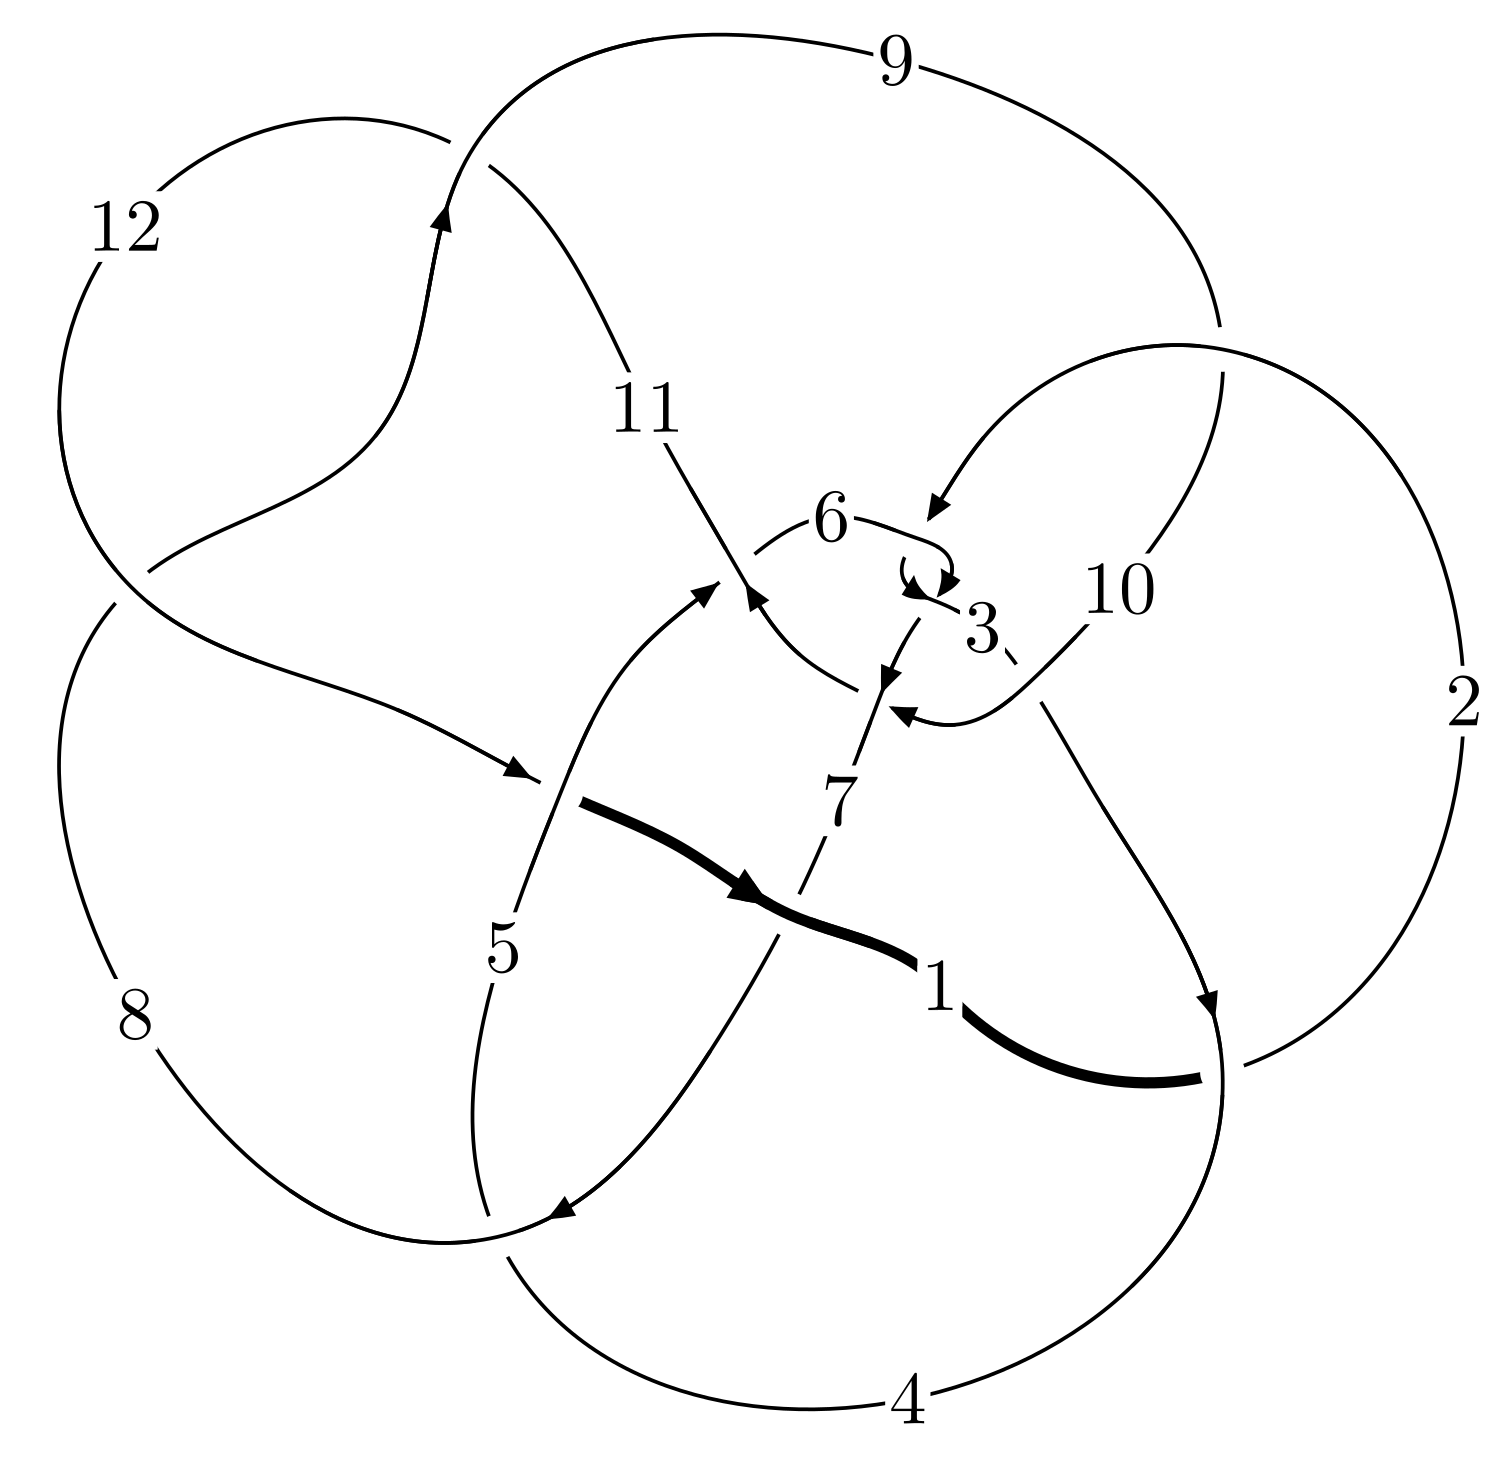
\includegraphics[width=112pt]{../../../GIT/diagram.site/Diagrams/png/1752_12a_0951.png}\\
\ \ \ A knot diagram\footnotemark}&
\allowdisplaybreaks
\textbf{Linearized knot diagam} \\
\cline{2-2}
 &
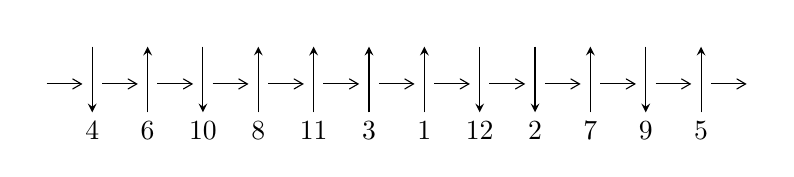
\begin{tikzpicture}[x=20pt, y=17pt]
	% nodes
	\node (C0) at (0, 0) {};
	\node (C1) at (1, 0) {};
	\node (C1U) at (1, +1) {};
	\node (C1D) at (1, -1) {4};

	\node (C2) at (2, 0) {};
	\node (C2U) at (2, +1) {};
	\node (C2D) at (2, -1) {6};

	\node (C3) at (3, 0) {};
	\node (C3U) at (3, +1) {};
	\node (C3D) at (3, -1) {10};

	\node (C4) at (4, 0) {};
	\node (C4U) at (4, +1) {};
	\node (C4D) at (4, -1) {8};

	\node (C5) at (5, 0) {};
	\node (C5U) at (5, +1) {};
	\node (C5D) at (5, -1) {11};

	\node (C6) at (6, 0) {};
	\node (C6U) at (6, +1) {};
	\node (C6D) at (6, -1) {3};

	\node (C7) at (7, 0) {};
	\node (C7U) at (7, +1) {};
	\node (C7D) at (7, -1) {1};

	\node (C8) at (8, 0) {};
	\node (C8U) at (8, +1) {};
	\node (C8D) at (8, -1) {12};

	\node (C9) at (9, 0) {};
	\node (C9U) at (9, +1) {};
	\node (C9D) at (9, -1) {2};

	\node (C10) at (10, 0) {};
	\node (C10U) at (10, +1) {};
	\node (C10D) at (10, -1) {7};

	\node (C11) at (11, 0) {};
	\node (C11U) at (11, +1) {};
	\node (C11D) at (11, -1) {9};

	\node (C12) at (12, 0) {};
	\node (C12U) at (12, +1) {};
	\node (C12D) at (12, -1) {5};
	\node (C13) at (13, 0) {};

	% arrows
	\draw[->,>={angle 60}]
	(C0) edge (C1) (C1) edge (C2) (C2) edge (C3) (C3) edge (C4) (C4) edge (C5) (C5) edge (C6) (C6) edge (C7) (C7) edge (C8) (C8) edge (C9) (C9) edge (C10) (C10) edge (C11) (C11) edge (C12) (C12) edge (C13) ;	\draw[->,>=stealth]
	(C1U) edge (C1D) (C2D) edge (C2U) (C3U) edge (C3D) (C4D) edge (C4U) (C5D) edge (C5U) (C6D) edge (C6U) (C7D) edge (C7U) (C8U) edge (C8D) (C9U) edge (C9D) (C10D) edge (C10U) (C11U) edge (C11D) (C12D) edge (C12U) ;
	\end{tikzpicture} \\
\hhline{~~} \\& 
\textbf{Solving Sequence} \\ \cline{2-2} 
 &
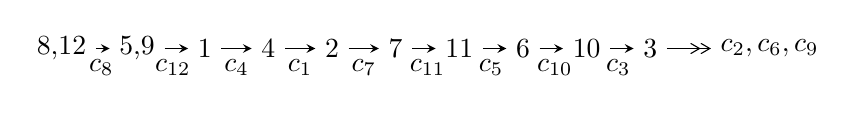
\begin{tikzpicture}[x=23pt, y=7pt]
	% node
	\node (A0) at (-1/8, 0) {8,12};
	\node (A1) at (17/16, 0) {5,9};
	\node (A2) at (17/8, 0) {1};
	\node (A3) at (25/8, 0) {4};
	\node (A4) at (33/8, 0) {2};
	\node (A5) at (41/8, 0) {7};
	\node (A6) at (49/8, 0) {11};
	\node (A7) at (57/8, 0) {6};
	\node (A8) at (65/8, 0) {10};
	\node (A9) at (73/8, 0) {3};
	\node (C1) at (1/2, -1) {$c_{8}$};
	\node (C2) at (13/8, -1) {$c_{12}$};
	\node (C3) at (21/8, -1) {$c_{4}$};
	\node (C4) at (29/8, -1) {$c_{1}$};
	\node (C5) at (37/8, -1) {$c_{7}$};
	\node (C6) at (45/8, -1) {$c_{11}$};
	\node (C7) at (53/8, -1) {$c_{5}$};
	\node (C8) at (61/8, -1) {$c_{10}$};
	\node (C9) at (69/8, -1) {$c_{3}$};
	\node (A10) at (11, 0) {$c_{2},c_{6},c_{9}$};

	% edge
	\draw[->,>=stealth]	
	(A0) edge (A1) (A1) edge (A2) (A2) edge (A3) (A3) edge (A4) (A4) edge (A5) (A5) edge (A6) (A6) edge (A7) (A7) edge (A8) (A8) edge (A9) ;
	\draw[->>,>={angle 60}]	
	(A9) edge (A10);
\end{tikzpicture} \\ 

\end{tabular} \\

\footnotetext{
The image of knot diagram is generated by the software ``\textbf{Draw programme}" developed by Andrew Bartholomew(\url{http://www.layer8.co.uk/maths/draw/index.htm\#Running-draw}), where we modified some parts for our purpose(\url{https://github.com/CATsTAILs/LinksPainter}).
}\phantom \\ \newline 
\centering \textbf{Ideals for irreducible components\footnotemark of $X_{\text{par}}$} 
 
\begin{align*}
I^u_{1}&=\langle 
-3.27230\times10^{1426} u^{193}+6.48474\times10^{1427} u^{192}+\cdots+2.85303\times10^{1429} b+7.63301\times10^{1432},\\
\phantom{I^u_{1}}&\phantom{= \langle  }-6.63186\times10^{1432} u^{193}+2.10738\times10^{1433} u^{192}+\cdots+4.49783\times10^{1434} a-1.59873\times10^{1438},\\
\phantom{I^u_{1}}&\phantom{= \langle  }u^{194}-5 u^{193}+\cdots-1119128 u+157651\rangle \\
I^u_{2}&=\langle 
-1.54069\times10^{49} u^{46}+1.60376\times10^{50} u^{45}+\cdots+5.91894\times10^{49} b-1.65232\times10^{50},\\
\phantom{I^u_{2}}&\phantom{= \langle  }-6.13499\times10^{50} u^{46}+7.39476\times10^{51} u^{45}+\cdots+5.91894\times10^{49} a-1.44700\times10^{52},\\
\phantom{I^u_{2}}&\phantom{= \langle  }u^{47}-12 u^{46}+\cdots+58 u-1\rangle \\
\\
\end{align*}
\raggedright * 2 irreducible components of $\dim_{\mathbb{C}}=0$, with total 241 representations.\\
\footnotetext{All coefficients of polynomials are rational numbers. But the coefficients are sometimes approximated in decimal forms when there is not enough margin.}
\newpage
\renewcommand{\arraystretch}{1}
\centering \section*{I. $I^u_{1}= \langle -3.27\times10^{1426} u^{193}+6.48\times10^{1427} u^{192}+\cdots+2.85\times10^{1429} b+7.63\times10^{1432},\;-6.63\times10^{1432} u^{193}+2.11\times10^{1433} u^{192}+\cdots+4.50\times10^{1434} a-1.60\times10^{1438},\;u^{194}-5 u^{193}+\cdots-1119128 u+157651 \rangle$}
\flushleft \textbf{(i) Arc colorings}\\
\begin{tabular}{m{7pt} m{180pt} m{7pt} m{180pt} }
\flushright $a_{8}=$&$\begin{pmatrix}1\\0\end{pmatrix}$ \\
\flushright $a_{12}=$&$\begin{pmatrix}0\\u\end{pmatrix}$ \\
\flushright $a_{5}=$&$\begin{pmatrix}0.0147446 u^{193}-0.0468534 u^{192}+\cdots-24069.2 u+3554.44\\0.00114696 u^{193}-0.0227293 u^{192}+\cdots+19755.5 u-2675.41\end{pmatrix}$ \\
\flushright $a_{9}=$&$\begin{pmatrix}1\\u^2\end{pmatrix}$ \\
\flushright $a_{1}=$&$\begin{pmatrix}0.00833197 u^{193}-0.0782035 u^{192}+\cdots+36715.7 u-4821.25\\0.0146802 u^{193}-0.0906046 u^{192}+\cdots+13746.0 u-1660.10\end{pmatrix}$ \\
\flushright $a_{4}=$&$\begin{pmatrix}0.0135976 u^{193}-0.0241240 u^{192}+\cdots-43824.8 u+6229.85\\0.00114696 u^{193}-0.0227293 u^{192}+\cdots+19755.5 u-2675.41\end{pmatrix}$ \\
\flushright $a_{2}=$&$\begin{pmatrix}0.0308401 u^{193}-0.276956 u^{192}+\cdots+121339. u-16125.2\\-0.00477786 u^{193}+0.124624 u^{192}+\cdots-99644.9 u+13722.4\end{pmatrix}$ \\
\flushright $a_{7}=$&$\begin{pmatrix}0.0172265 u^{193}-0.0100294 u^{192}+\cdots-83320.6 u+11703.9\\-0.0220203 u^{193}+0.0900415 u^{192}+\cdots+26764.2 u-4108.74\end{pmatrix}$ \\
\flushright $a_{11}=$&$\begin{pmatrix}u\\u^3+u\end{pmatrix}$ \\
\flushright $a_{6}=$&$\begin{pmatrix}0.00495432 u^{193}+0.0150898 u^{192}+\cdots-40759.3 u+5655.43\\-0.000435455 u^{193}-0.0130372 u^{192}+\cdots+19148.5 u-2622.59\end{pmatrix}$ \\
\flushright $a_{10}=$&$\begin{pmatrix}0.174327 u^{193}-0.948024 u^{192}+\cdots+74897.4 u-7006.96\\-0.0195033 u^{193}+0.214641 u^{192}+\cdots-118724. u+16042.2\end{pmatrix}$ \\
\flushright $a_{3}=$&$\begin{pmatrix}0.0328154 u^{193}-0.211872 u^{192}+\cdots+51155.0 u-6320.11\\-0.00238623 u^{193}+0.00592457 u^{192}+\cdots+1963.76 u-309.126\end{pmatrix}$\\&\end{tabular}
\flushleft \textbf{(ii) Obstruction class $= -1$}\\~\\
\flushleft \textbf{(iii) Cusp Shapes $= -0.144687 u^{193}+0.778133 u^{192}+\cdots-43152.8 u+3187.26$}\\~\\
\newpage\renewcommand{\arraystretch}{1}
\flushleft \textbf{(iv) u-Polynomials at the component}\newline \\
\begin{tabular}{m{50pt}|m{274pt}}
Crossings & \hspace{64pt}u-Polynomials at each crossing \\
\hline $$\begin{aligned}c_{1}\end{aligned}$$&$\begin{aligned}
&u^{194}-15 u^{193}+\cdots+4276480 u-140732
\end{aligned}$\\
\hline $$\begin{aligned}c_{2},c_{6}\end{aligned}$$&$\begin{aligned}
&u^{194}-2 u^{193}+\cdots-115 u+763
\end{aligned}$\\
\hline $$\begin{aligned}c_{3}\end{aligned}$$&$\begin{aligned}
&u^{194}-3 u^{193}+\cdots+10121514 u-2950781
\end{aligned}$\\
\hline $$\begin{aligned}c_{4}\end{aligned}$$&$\begin{aligned}
&u^{194}-5 u^{193}+\cdots-1229250 u-450361
\end{aligned}$\\
\hline $$\begin{aligned}c_{5}\end{aligned}$$&$\begin{aligned}
&u^{194}-3 u^{193}+\cdots+1930268 u-110863
\end{aligned}$\\
\hline $$\begin{aligned}c_{7}\end{aligned}$$&$\begin{aligned}
&u^{194}+3 u^{193}+\cdots+39 u+1
\end{aligned}$\\
\hline $$\begin{aligned}c_{8},c_{11}\end{aligned}$$&$\begin{aligned}
&u^{194}+5 u^{193}+\cdots+1119128 u+157651
\end{aligned}$\\
\hline $$\begin{aligned}c_{9}\end{aligned}$$&$\begin{aligned}
&u^{194}-2 u^{193}+\cdots+29446983 u-7136263
\end{aligned}$\\
\hline $$\begin{aligned}c_{10}\end{aligned}$$&$\begin{aligned}
&u^{194}-6 u^{193}+\cdots-4089433 u+368299
\end{aligned}$\\
\hline $$\begin{aligned}c_{12}\end{aligned}$$&$\begin{aligned}
&u^{194}-3 u^{193}+\cdots-1779 u-187
\end{aligned}$\\
\hline
\end{tabular}\\~\\
\newpage\renewcommand{\arraystretch}{1}
\flushleft \textbf{(v) Riley Polynomials at the component}\newline \\
\begin{tabular}{m{50pt}|m{274pt}}
Crossings & \hspace{64pt}Riley Polynomials at each crossing \\
\hline $$\begin{aligned}c_{1}\end{aligned}$$&$\begin{aligned}
&y^{194}+57 y^{193}+\cdots+9871873955280 y+19805495824
\end{aligned}$\\
\hline $$\begin{aligned}c_{2},c_{6}\end{aligned}$$&$\begin{aligned}
&y^{194}-122 y^{193}+\cdots-27508693 y+582169
\end{aligned}$\\
\hline $$\begin{aligned}c_{3}\end{aligned}$$&$\begin{aligned}
&y^{194}+43 y^{193}+\cdots-281074639663414 y+8707108509961
\end{aligned}$\\
\hline $$\begin{aligned}c_{4}\end{aligned}$$&$\begin{aligned}
&y^{194}-49 y^{193}+\cdots-4233488708222 y+202825030321
\end{aligned}$\\
\hline $$\begin{aligned}c_{5}\end{aligned}$$&$\begin{aligned}
&y^{194}+9 y^{193}+\cdots-1148717911644 y+12290604769
\end{aligned}$\\
\hline $$\begin{aligned}c_{7}\end{aligned}$$&$\begin{aligned}
&y^{194}+11 y^{193}+\cdots-137 y+1
\end{aligned}$\\
\hline $$\begin{aligned}c_{8},c_{11}\end{aligned}$$&$\begin{aligned}
&y^{194}+145 y^{193}+\cdots-983610590218 y+24853837801
\end{aligned}$\\
\hline $$\begin{aligned}c_{9}\end{aligned}$$&$\begin{aligned}
&y^{194}+70 y^{193}+\cdots+2458572666392573 y+50926249605169
\end{aligned}$\\
\hline $$\begin{aligned}c_{10}\end{aligned}$$&$\begin{aligned}
&y^{194}-20 y^{193}+\cdots-11280170985833 y+135644153401
\end{aligned}$\\
\hline $$\begin{aligned}c_{12}\end{aligned}$$&$\begin{aligned}
&y^{194}-31 y^{193}+\cdots-837813 y+34969
\end{aligned}$\\
\hline
\end{tabular}\\~\\
\newpage\flushleft \textbf{(vi) Complex Volumes and Cusp Shapes}
$$\begin{array}{c|c|c}  
\text{Solutions to }I^u_{1}& \I (\text{vol} + \sqrt{-1}CS) & \text{Cusp shape}\\
 \hline 
\begin{aligned}
u &= -0.384187 + 0.923055 I \\
a &= \phantom{-}0.53775 - 1.59785 I \\
b &= -0.805099 - 0.707456 I\end{aligned}
 & \phantom{-}0.882578 - 0.354022 I & \phantom{-0.000000 } 0 \\ \hline\begin{aligned}
u &= -0.384187 - 0.923055 I \\
a &= \phantom{-}0.53775 + 1.59785 I \\
b &= -0.805099 + 0.707456 I\end{aligned}
 & \phantom{-}0.882578 + 0.354022 I & \phantom{-0.000000 } 0 \\ \hline\begin{aligned}
u &= \phantom{-}0.547871 + 0.829575 I \\
a &= -0.354733 + 0.297690 I \\
b &= \phantom{-}2.06672 + 1.19986 I\end{aligned}
 & \phantom{-}1.28330 - 2.18942 I & \phantom{-0.000000 } 0 \\ \hline\begin{aligned}
u &= \phantom{-}0.547871 - 0.829575 I \\
a &= -0.354733 - 0.297690 I \\
b &= \phantom{-}2.06672 - 1.19986 I\end{aligned}
 & \phantom{-}1.28330 + 2.18942 I & \phantom{-0.000000 } 0 \\ \hline\begin{aligned}
u &= -0.209765 + 0.961427 I \\
a &= \phantom{-}0.65792 - 1.31308 I \\
b &= -1.29266 - 0.70184 I\end{aligned}
 & \phantom{-}5.17068 + 4.36065 I & \phantom{-0.000000 } 0 \\ \hline\begin{aligned}
u &= -0.209765 - 0.961427 I \\
a &= \phantom{-}0.65792 + 1.31308 I \\
b &= -1.29266 + 0.70184 I\end{aligned}
 & \phantom{-}5.17068 - 4.36065 I & \phantom{-0.000000 } 0 \\ \hline\begin{aligned}
u &= -0.067146 + 0.979563 I \\
a &= -1.207000 + 0.288332 I \\
b &= \phantom{-}1.65912 + 0.33912 I\end{aligned}
 & -1.39515 + 2.23030 I & \phantom{-0.000000 } 0 \\ \hline\begin{aligned}
u &= -0.067146 - 0.979563 I \\
a &= -1.207000 - 0.288332 I \\
b &= \phantom{-}1.65912 - 0.33912 I\end{aligned}
 & -1.39515 - 2.23030 I & \phantom{-0.000000 } 0 \\ \hline\begin{aligned}
u &= \phantom{-}0.929594 + 0.230082 I \\
a &= -0.075912 - 0.942965 I \\
b &= \phantom{-}0.446309 - 0.753113 I\end{aligned}
 & -1.90842 - 1.54765 I & \phantom{-0.000000 } 0 \\ \hline\begin{aligned}
u &= \phantom{-}0.929594 - 0.230082 I \\
a &= -0.075912 + 0.942965 I \\
b &= \phantom{-}0.446309 + 0.753113 I\end{aligned}
 & -1.90842 + 1.54765 I & \phantom{-0.000000 } 0\\
 \hline 
 \end{array}$$\newpage$$\begin{array}{c|c|c}  
\text{Solutions to }I^u_{1}& \I (\text{vol} + \sqrt{-1}CS) & \text{Cusp shape}\\
 \hline 
\begin{aligned}
u &= -0.317208 + 0.993886 I \\
a &= \phantom{-}0.248922 - 0.356553 I \\
b &= \phantom{-}0.37881 - 1.87980 I\end{aligned}
 & \phantom{-}0.40586 + 6.78834 I & \phantom{-0.000000 } 0 \\ \hline\begin{aligned}
u &= -0.317208 - 0.993886 I \\
a &= \phantom{-}0.248922 + 0.356553 I \\
b &= \phantom{-}0.37881 + 1.87980 I\end{aligned}
 & \phantom{-}0.40586 - 6.78834 I & \phantom{-0.000000 } 0 \\ \hline\begin{aligned}
u &= -0.133115 + 1.035690 I \\
a &= \phantom{-}1.42681 - 0.39663 I \\
b &= -1.54051 - 0.24913 I\end{aligned}
 & \phantom{-}2.39749 + 7.47414 I & \phantom{-0.000000 } 0 \\ \hline\begin{aligned}
u &= -0.133115 - 1.035690 I \\
a &= \phantom{-}1.42681 + 0.39663 I \\
b &= -1.54051 + 0.24913 I\end{aligned}
 & \phantom{-}2.39749 - 7.47414 I & \phantom{-0.000000 } 0 \\ \hline\begin{aligned}
u &= \phantom{-}0.909210 + 0.258622 I \\
a &= -0.366460 - 0.752034 I \\
b &= -0.068197 - 0.805149 I\end{aligned}
 & -1.87235 - 1.23811 I & \phantom{-0.000000 } 0 \\ \hline\begin{aligned}
u &= \phantom{-}0.909210 - 0.258622 I \\
a &= -0.366460 + 0.752034 I \\
b &= -0.068197 + 0.805149 I\end{aligned}
 & -1.87235 + 1.23811 I & \phantom{-0.000000 } 0 \\ \hline\begin{aligned}
u &= \phantom{-}0.322789 + 1.004590 I \\
a &= \phantom{-}0.115468 + 0.516083 I \\
b &= \phantom{-}0.381496 + 0.979514 I\end{aligned}
 & \phantom{-}0.47698 - 2.62744 I & \phantom{-0.000000 } 0 \\ \hline\begin{aligned}
u &= \phantom{-}0.322789 - 1.004590 I \\
a &= \phantom{-}0.115468 - 0.516083 I \\
b &= \phantom{-}0.381496 - 0.979514 I\end{aligned}
 & \phantom{-}0.47698 + 2.62744 I & \phantom{-0.000000 } 0 \\ \hline\begin{aligned}
u &= -0.970856 + 0.442065 I \\
a &= \phantom{-}0.678964 + 0.191918 I \\
b &= \phantom{-}0.740155 - 0.339848 I\end{aligned}
 & \phantom{-}5.49512 - 3.29198 I & \phantom{-0.000000 } 0 \\ \hline\begin{aligned}
u &= -0.970856 - 0.442065 I \\
a &= \phantom{-}0.678964 - 0.191918 I \\
b &= \phantom{-}0.740155 + 0.339848 I\end{aligned}
 & \phantom{-}5.49512 + 3.29198 I & \phantom{-0.000000 } 0\\
 \hline 
 \end{array}$$\newpage$$\begin{array}{c|c|c}  
\text{Solutions to }I^u_{1}& \I (\text{vol} + \sqrt{-1}CS) & \text{Cusp shape}\\
 \hline 
\begin{aligned}
u &= -0.100011 + 1.073050 I \\
a &= -0.43422 + 1.88249 I \\
b &= \phantom{-}0.909644 + 0.229531 I\end{aligned}
 & \phantom{-}9.38363 + 0.54889 I & \phantom{-0.000000 } 0 \\ \hline\begin{aligned}
u &= -0.100011 - 1.073050 I \\
a &= -0.43422 - 1.88249 I \\
b &= \phantom{-}0.909644 - 0.229531 I\end{aligned}
 & \phantom{-}9.38363 - 0.54889 I & \phantom{-0.000000 } 0 \\ \hline\begin{aligned}
u &= \phantom{-}0.183561 + 1.062180 I \\
a &= \phantom{-}0.808569 - 0.277045 I \\
b &= -1.74530 - 0.46331 I\end{aligned}
 & \phantom{-}3.45076 - 1.76457 I & \phantom{-0.000000 } 0 \\ \hline\begin{aligned}
u &= \phantom{-}0.183561 - 1.062180 I \\
a &= \phantom{-}0.808569 + 0.277045 I \\
b &= -1.74530 + 0.46331 I\end{aligned}
 & \phantom{-}3.45076 + 1.76457 I & \phantom{-0.000000 } 0 \\ \hline\begin{aligned}
u &= \phantom{-}0.727729 + 0.558414 I \\
a &= -0.411433 - 0.800613 I \\
b &= \phantom{-}0.840718 - 0.714335 I\end{aligned}
 & -1.56282 - 1.54817 I & \phantom{-0.000000 } 0 \\ \hline\begin{aligned}
u &= \phantom{-}0.727729 - 0.558414 I \\
a &= -0.411433 + 0.800613 I \\
b &= \phantom{-}0.840718 + 0.714335 I\end{aligned}
 & -1.56282 + 1.54817 I & \phantom{-0.000000 } 0 \\ \hline\begin{aligned}
u &= -0.021838 + 1.083020 I \\
a &= -0.87788 + 1.16124 I \\
b &= \phantom{-}1.32343 + 0.68730 I\end{aligned}
 & \phantom{-}6.20464 + 3.83618 I & \phantom{-0.000000 } 0 \\ \hline\begin{aligned}
u &= -0.021838 - 1.083020 I \\
a &= -0.87788 - 1.16124 I \\
b &= \phantom{-}1.32343 - 0.68730 I\end{aligned}
 & \phantom{-}6.20464 - 3.83618 I & \phantom{-0.000000 } 0 \\ \hline\begin{aligned}
u &= \phantom{-}0.588558 + 0.909939 I \\
a &= -0.067213 + 0.364998 I \\
b &= -0.01545 + 1.58534 I\end{aligned}
 & \phantom{-}1.00993 - 2.04639 I & \phantom{-0.000000 } 0 \\ \hline\begin{aligned}
u &= \phantom{-}0.588558 - 0.909939 I \\
a &= -0.067213 - 0.364998 I \\
b &= -0.01545 - 1.58534 I\end{aligned}
 & \phantom{-}1.00993 + 2.04639 I & \phantom{-0.000000 } 0\\
 \hline 
 \end{array}$$\newpage$$\begin{array}{c|c|c}  
\text{Solutions to }I^u_{1}& \I (\text{vol} + \sqrt{-1}CS) & \text{Cusp shape}\\
 \hline 
\begin{aligned}
u &= \phantom{-}0.093755 + 1.088810 I \\
a &= \phantom{-}0.94274 - 1.31144 I \\
b &= -0.741405 - 0.260404 I\end{aligned}
 & \phantom{-}3.22267 - 0.45617 I & \phantom{-0.000000 } 0 \\ \hline\begin{aligned}
u &= \phantom{-}0.093755 - 1.088810 I \\
a &= \phantom{-}0.94274 + 1.31144 I \\
b &= -0.741405 + 0.260404 I\end{aligned}
 & \phantom{-}3.22267 + 0.45617 I & \phantom{-0.000000 } 0 \\ \hline\begin{aligned}
u &= -0.106457 + 1.097550 I \\
a &= -0.149029 + 0.249252 I \\
b &= -0.50404 + 1.96691 I\end{aligned}
 & \phantom{-}5.84091 + 0.86513 I & \phantom{-0.000000 } 0 \\ \hline\begin{aligned}
u &= -0.106457 - 1.097550 I \\
a &= -0.149029 - 0.249252 I \\
b &= -0.50404 - 1.96691 I\end{aligned}
 & \phantom{-}5.84091 - 0.86513 I & \phantom{-0.000000 } 0 \\ \hline\begin{aligned}
u &= -0.024652 + 1.103430 I \\
a &= -0.235632 - 0.868158 I \\
b &= \phantom{-}1.10516 - 1.63869 I\end{aligned}
 & \phantom{-}6.52151 + 0.51104 I & \phantom{-0.000000 } 0 \\ \hline\begin{aligned}
u &= -0.024652 - 1.103430 I \\
a &= -0.235632 + 0.868158 I \\
b &= \phantom{-}1.10516 + 1.63869 I\end{aligned}
 & \phantom{-}6.52151 - 0.51104 I & \phantom{-0.000000 } 0 \\ \hline\begin{aligned}
u &= -0.806229 + 0.390588 I \\
a &= -0.715276 - 0.623908 I \\
b &= -0.832062 - 0.493893 I\end{aligned}
 & \phantom{-}1.65776 - 0.16374 I & \phantom{-0.000000 } 0 \\ \hline\begin{aligned}
u &= -0.806229 - 0.390588 I \\
a &= -0.715276 + 0.623908 I \\
b &= -0.832062 + 0.493893 I\end{aligned}
 & \phantom{-}1.65776 + 0.16374 I & \phantom{-0.000000 } 0 \\ \hline\begin{aligned}
u &= \phantom{-}0.428627 + 0.784720 I \\
a &= -0.22687 + 1.60637 I \\
b &= -0.789215 + 0.751485 I\end{aligned}
 & \phantom{-}0.53364 - 5.06652 I & \phantom{-0.000000 } 0 \\ \hline\begin{aligned}
u &= \phantom{-}0.428627 - 0.784720 I \\
a &= -0.22687 - 1.60637 I \\
b &= -0.789215 - 0.751485 I\end{aligned}
 & \phantom{-}0.53364 + 5.06652 I & \phantom{-0.000000 } 0\\
 \hline 
 \end{array}$$\newpage$$\begin{array}{c|c|c}  
\text{Solutions to }I^u_{1}& \I (\text{vol} + \sqrt{-1}CS) & \text{Cusp shape}\\
 \hline 
\begin{aligned}
u &= -0.697781 + 0.548563 I \\
a &= -1.136800 + 0.567887 I \\
b &= -0.598221 + 0.555474 I\end{aligned}
 & -0.31010 + 4.61607 I & \phantom{-0.000000 } 0 \\ \hline\begin{aligned}
u &= -0.697781 - 0.548563 I \\
a &= -1.136800 - 0.567887 I \\
b &= -0.598221 - 0.555474 I\end{aligned}
 & -0.31010 - 4.61607 I & \phantom{-0.000000 } 0 \\ \hline\begin{aligned}
u &= -0.113001 + 1.110790 I \\
a &= \phantom{-}1.46316 + 1.42866 I \\
b &= -0.591997 - 0.029070 I\end{aligned}
 & \phantom{-}2.88948 + 5.70871 I & \phantom{-0.000000 } 0 \\ \hline\begin{aligned}
u &= -0.113001 - 1.110790 I \\
a &= \phantom{-}1.46316 - 1.42866 I \\
b &= -0.591997 + 0.029070 I\end{aligned}
 & \phantom{-}2.88948 - 5.70871 I & \phantom{-0.000000 } 0 \\ \hline\begin{aligned}
u &= \phantom{-}0.184699 + 1.106530 I \\
a &= \phantom{-}0.478732 + 0.748414 I \\
b &= -1.74322 + 1.17361 I\end{aligned}
 & \phantom{-}3.96498 - 6.97076 I & \phantom{-0.000000 } 0 \\ \hline\begin{aligned}
u &= \phantom{-}0.184699 - 1.106530 I \\
a &= \phantom{-}0.478732 - 0.748414 I \\
b &= -1.74322 - 1.17361 I\end{aligned}
 & \phantom{-}3.96498 + 6.97076 I & \phantom{-0.000000 } 0 \\ \hline\begin{aligned}
u &= \phantom{-}1.128180 + 0.151128 I \\
a &= \phantom{-}0.607242 + 0.594696 I \\
b &= \phantom{-}0.783317 + 0.563490 I\end{aligned}
 & -1.30042 + 3.17379 I & \phantom{-0.000000 } 0 \\ \hline\begin{aligned}
u &= \phantom{-}1.128180 - 0.151128 I \\
a &= \phantom{-}0.607242 - 0.594696 I \\
b &= \phantom{-}0.783317 - 0.563490 I\end{aligned}
 & -1.30042 - 3.17379 I & \phantom{-0.000000 } 0 \\ \hline\begin{aligned}
u &= -0.268237 + 0.805354 I \\
a &= \phantom{-}0.327458 + 1.047400 I \\
b &= \phantom{-}0.873437 - 0.213738 I\end{aligned}
 & \phantom{-}5.12044 - 3.25393 I & \phantom{-0.000000 } 0 \\ \hline\begin{aligned}
u &= -0.268237 - 0.805354 I \\
a &= \phantom{-}0.327458 - 1.047400 I \\
b &= \phantom{-}0.873437 + 0.213738 I\end{aligned}
 & \phantom{-}5.12044 + 3.25393 I & \phantom{-0.000000 } 0\\
 \hline 
 \end{array}$$\newpage$$\begin{array}{c|c|c}  
\text{Solutions to }I^u_{1}& \I (\text{vol} + \sqrt{-1}CS) & \text{Cusp shape}\\
 \hline 
\begin{aligned}
u &= -0.410483 + 1.081760 I \\
a &= -0.186288 + 0.393603 I \\
b &= -0.45581 + 1.88365 I\end{aligned}
 & \phantom{-}4.42633 + 12.80160 I & \phantom{-0.000000 } 0 \\ \hline\begin{aligned}
u &= -0.410483 - 1.081760 I \\
a &= -0.186288 - 0.393603 I \\
b &= -0.45581 - 1.88365 I\end{aligned}
 & \phantom{-}4.42633 - 12.80160 I & \phantom{-0.000000 } 0 \\ \hline\begin{aligned}
u &= \phantom{-}0.106512 + 1.153680 I \\
a &= -0.61325 - 1.89560 I \\
b &= \phantom{-}0.602464 - 0.150181 I\end{aligned}
 & \phantom{-}8.66222 - 0.88413 I & \phantom{-0.000000 } 0 \\ \hline\begin{aligned}
u &= \phantom{-}0.106512 - 1.153680 I \\
a &= -0.61325 + 1.89560 I \\
b &= \phantom{-}0.602464 + 0.150181 I\end{aligned}
 & \phantom{-}8.66222 + 0.88413 I & \phantom{-0.000000 } 0 \\ \hline\begin{aligned}
u &= \phantom{-}0.272154 + 1.132360 I \\
a &= \phantom{-}0.08019 - 1.70009 I \\
b &= \phantom{-}0.705381 - 0.131388 I\end{aligned}
 & \phantom{-}8.57265 - 0.97336 I & \phantom{-0.000000 } 0 \\ \hline\begin{aligned}
u &= \phantom{-}0.272154 - 1.132360 I \\
a &= \phantom{-}0.08019 + 1.70009 I \\
b &= \phantom{-}0.705381 + 0.131388 I\end{aligned}
 & \phantom{-}8.57265 + 0.97336 I & \phantom{-0.000000 } 0 \\ \hline\begin{aligned}
u &= -1.165750 + 0.016804 I \\
a &= \phantom{-}0.612918 + 0.717723 I \\
b &= \phantom{-}0.909049 + 0.816394 I\end{aligned}
 & -1.26176 + 9.55015 I & \phantom{-0.000000 } 0 \\ \hline\begin{aligned}
u &= -1.165750 - 0.016804 I \\
a &= \phantom{-}0.612918 - 0.717723 I \\
b &= \phantom{-}0.909049 - 0.816394 I\end{aligned}
 & -1.26176 - 9.55015 I & \phantom{-0.000000 } 0 \\ \hline\begin{aligned}
u &= -0.187968 + 1.153950 I \\
a &= \phantom{-}1.41627 + 0.02807 I \\
b &= -0.858920 - 0.338392 I\end{aligned}
 & \phantom{-}6.19578 + 3.16235 I & \phantom{-0.000000 } 0 \\ \hline\begin{aligned}
u &= -0.187968 - 1.153950 I \\
a &= \phantom{-}1.41627 - 0.02807 I \\
b &= -0.858920 + 0.338392 I\end{aligned}
 & \phantom{-}6.19578 - 3.16235 I & \phantom{-0.000000 } 0\\
 \hline 
 \end{array}$$\newpage$$\begin{array}{c|c|c}  
\text{Solutions to }I^u_{1}& \I (\text{vol} + \sqrt{-1}CS) & \text{Cusp shape}\\
 \hline 
\begin{aligned}
u &= \phantom{-}0.046994 + 1.174320 I \\
a &= \phantom{-}0.356754 - 1.000260 I \\
b &= -0.901498 - 0.025037 I\end{aligned}
 & \phantom{-}6.84747 - 3.47433 I & \phantom{-0.000000 } 0 \\ \hline\begin{aligned}
u &= \phantom{-}0.046994 - 1.174320 I \\
a &= \phantom{-}0.356754 + 1.000260 I \\
b &= -0.901498 + 0.025037 I\end{aligned}
 & \phantom{-}6.84747 + 3.47433 I & \phantom{-0.000000 } 0 \\ \hline\begin{aligned}
u &= -0.360883 + 1.119560 I \\
a &= -0.58212 + 1.33785 I \\
b &= \phantom{-}0.944194 + 0.894544 I\end{aligned}
 & -1.74834 + 5.54437 I & \phantom{-0.000000 } 0 \\ \hline\begin{aligned}
u &= -0.360883 - 1.119560 I \\
a &= -0.58212 - 1.33785 I \\
b &= \phantom{-}0.944194 - 0.894544 I\end{aligned}
 & -1.74834 - 5.54437 I & \phantom{-0.000000 } 0 \\ \hline\begin{aligned}
u &= \phantom{-}1.175870 + 0.039345 I \\
a &= -0.301766 + 0.532082 I \\
b &= -0.837138 + 0.991374 I\end{aligned}
 & -0.63520 - 2.80694 I & \phantom{-0.000000 } 0 \\ \hline\begin{aligned}
u &= \phantom{-}1.175870 - 0.039345 I \\
a &= -0.301766 - 0.532082 I \\
b &= -0.837138 - 0.991374 I\end{aligned}
 & -0.63520 + 2.80694 I & \phantom{-0.000000 } 0 \\ \hline\begin{aligned}
u &= -0.710347 + 0.406679 I \\
a &= \phantom{-}0.824024 - 0.834864 I \\
b &= -1.07466 - 0.93656 I\end{aligned}
 & \phantom{-}2.38127 - 8.54256 I & \phantom{-0.000000 } 0 \\ \hline\begin{aligned}
u &= -0.710347 - 0.406679 I \\
a &= \phantom{-}0.824024 + 0.834864 I \\
b &= -1.07466 + 0.93656 I\end{aligned}
 & \phantom{-}2.38127 + 8.54256 I & \phantom{-0.000000 } 0 \\ \hline\begin{aligned}
u &= -0.190968 + 1.172120 I \\
a &= -1.33436 - 1.24094 I \\
b &= \phantom{-}0.654821 + 0.028846 I\end{aligned}
 & \phantom{-}7.14634 + 11.85640 I & \phantom{-0.000000 } 0 \\ \hline\begin{aligned}
u &= -0.190968 - 1.172120 I \\
a &= -1.33436 + 1.24094 I \\
b &= \phantom{-}0.654821 - 0.028846 I\end{aligned}
 & \phantom{-}7.14634 - 11.85640 I & \phantom{-0.000000 } 0\\
 \hline 
 \end{array}$$\newpage$$\begin{array}{c|c|c}  
\text{Solutions to }I^u_{1}& \I (\text{vol} + \sqrt{-1}CS) & \text{Cusp shape}\\
 \hline 
\begin{aligned}
u &= \phantom{-}0.665458 + 0.984766 I \\
a &= \phantom{-}0.228943 + 0.394990 I \\
b &= -0.088578 + 0.984599 I\end{aligned}
 & -0.11278 - 4.00020 I & \phantom{-0.000000 } 0 \\ \hline\begin{aligned}
u &= \phantom{-}0.665458 - 0.984766 I \\
a &= \phantom{-}0.228943 - 0.394990 I \\
b &= -0.088578 - 0.984599 I\end{aligned}
 & -0.11278 + 4.00020 I & \phantom{-0.000000 } 0 \\ \hline\begin{aligned}
u &= -0.026484 + 1.199200 I \\
a &= \phantom{-}0.037826 + 0.244754 I \\
b &= -1.73820 + 0.38167 I\end{aligned}
 & \phantom{-}5.71665 + 5.06428 I & \phantom{-0.000000 } 0 \\ \hline\begin{aligned}
u &= -0.026484 - 1.199200 I \\
a &= \phantom{-}0.037826 - 0.244754 I \\
b &= -1.73820 - 0.38167 I\end{aligned}
 & \phantom{-}5.71665 - 5.06428 I & \phantom{-0.000000 } 0 \\ \hline\begin{aligned}
u &= -0.302106 + 1.168640 I \\
a &= -0.583894 + 1.223100 I \\
b &= \phantom{-}0.851712 + 1.128200 I\end{aligned}
 & -1.43312 + 5.51895 I & \phantom{-0.000000 } 0 \\ \hline\begin{aligned}
u &= -0.302106 - 1.168640 I \\
a &= -0.583894 - 1.223100 I \\
b &= \phantom{-}0.851712 - 1.128200 I\end{aligned}
 & -1.43312 - 5.51895 I & \phantom{-0.000000 } 0 \\ \hline\begin{aligned}
u &= \phantom{-}0.418811 + 1.143070 I \\
a &= \phantom{-}0.231939 + 0.871884 I \\
b &= -0.593553 + 0.995363 I\end{aligned}
 & \phantom{-}0.76686 - 3.40450 I & \phantom{-0.000000 } 0 \\ \hline\begin{aligned}
u &= \phantom{-}0.418811 - 1.143070 I \\
a &= \phantom{-}0.231939 - 0.871884 I \\
b &= -0.593553 - 0.995363 I\end{aligned}
 & \phantom{-}0.76686 + 3.40450 I & \phantom{-0.000000 } 0 \\ \hline\begin{aligned}
u &= -0.768396 + 0.123348 I \\
a &= -0.88816 - 1.14852 I \\
b &= -0.983151 - 0.737691 I\end{aligned}
 & \phantom{-}4.04348 + 5.09661 I & \phantom{-0.000000 } 0 \\ \hline\begin{aligned}
u &= -0.768396 - 0.123348 I \\
a &= -0.88816 + 1.14852 I \\
b &= -0.983151 + 0.737691 I\end{aligned}
 & \phantom{-}4.04348 - 5.09661 I & \phantom{-0.000000 } 0\\
 \hline 
 \end{array}$$\newpage$$\begin{array}{c|c|c}  
\text{Solutions to }I^u_{1}& \I (\text{vol} + \sqrt{-1}CS) & \text{Cusp shape}\\
 \hline 
\begin{aligned}
u &= \phantom{-}1.211190 + 0.219967 I \\
a &= \phantom{-}0.207834 - 0.710594 I \\
b &= \phantom{-}0.998430 - 0.907812 I\end{aligned}
 & -0.80913 - 4.70060 I & \phantom{-0.000000 } 0 \\ \hline\begin{aligned}
u &= \phantom{-}1.211190 - 0.219967 I \\
a &= \phantom{-}0.207834 + 0.710594 I \\
b &= \phantom{-}0.998430 + 0.907812 I\end{aligned}
 & -0.80913 + 4.70060 I & \phantom{-0.000000 } 0 \\ \hline\begin{aligned}
u &= -0.016601 + 1.237330 I \\
a &= \phantom{-}0.372544 - 1.192730 I \\
b &= -0.295113 - 1.151430 I\end{aligned}
 & \phantom{-}5.98313 - 0.93238 I & \phantom{-0.000000 } 0 \\ \hline\begin{aligned}
u &= -0.016601 - 1.237330 I \\
a &= \phantom{-}0.372544 + 1.192730 I \\
b &= -0.295113 + 1.151430 I\end{aligned}
 & \phantom{-}5.98313 + 0.93238 I & \phantom{-0.000000 } 0 \\ \hline\begin{aligned}
u &= -0.760502 + 0.009749 I \\
a &= -0.98454 + 1.42877 I \\
b &= -0.489014 + 0.715572 I\end{aligned}
 & -0.97472 - 8.07711 I & \phantom{-0.000000 } 0 \\ \hline\begin{aligned}
u &= -0.760502 - 0.009749 I \\
a &= -0.98454 - 1.42877 I \\
b &= -0.489014 - 0.715572 I\end{aligned}
 & -0.97472 + 8.07711 I & \phantom{-0.000000 } 0 \\ \hline\begin{aligned}
u &= -0.625148 + 0.422116 I \\
a &= \phantom{-}1.36027 - 0.57232 I \\
b &= \phantom{-}0.700287 - 0.717317 I\end{aligned}
 & -3.98732 - 1.76256 I & \phantom{-0.000000 } 0 \\ \hline\begin{aligned}
u &= -0.625148 - 0.422116 I \\
a &= \phantom{-}1.36027 + 0.57232 I \\
b &= \phantom{-}0.700287 + 0.717317 I\end{aligned}
 & -3.98732 + 1.76256 I & \phantom{-0.000000 } 0 \\ \hline\begin{aligned}
u &= \phantom{-}0.480325 + 1.153660 I \\
a &= \phantom{-}0.021123 - 0.311255 I \\
b &= \phantom{-}0.04944 - 1.63014 I\end{aligned}
 & \phantom{-}2.18953 - 3.09823 I & \phantom{-0.000000 } 0 \\ \hline\begin{aligned}
u &= \phantom{-}0.480325 - 1.153660 I \\
a &= \phantom{-}0.021123 + 0.311255 I \\
b &= \phantom{-}0.04944 + 1.63014 I\end{aligned}
 & \phantom{-}2.18953 + 3.09823 I & \phantom{-0.000000 } 0\\
 \hline 
 \end{array}$$\newpage$$\begin{array}{c|c|c}  
\text{Solutions to }I^u_{1}& \I (\text{vol} + \sqrt{-1}CS) & \text{Cusp shape}\\
 \hline 
\begin{aligned}
u &= \phantom{-}0.072535 + 1.251720 I \\
a &= -1.286300 - 0.585761 I \\
b &= \phantom{-}0.714844 - 0.016193 I\end{aligned}
 & \phantom{-}4.31899 - 2.92255 I & \phantom{-0.000000 } 0 \\ \hline\begin{aligned}
u &= \phantom{-}0.072535 - 1.251720 I \\
a &= -1.286300 + 0.585761 I \\
b &= \phantom{-}0.714844 + 0.016193 I\end{aligned}
 & \phantom{-}4.31899 + 2.92255 I & \phantom{-0.000000 } 0 \\ \hline\begin{aligned}
u &= -0.082900 + 0.727312 I \\
a &= \phantom{-}0.254407 - 0.031281 I \\
b &= \phantom{-}0.871211 - 0.957883 I\end{aligned}
 & -1.89677 - 1.12936 I & \phantom{-0.000000 } 0 \\ \hline\begin{aligned}
u &= -0.082900 - 0.727312 I \\
a &= \phantom{-}0.254407 + 0.031281 I \\
b &= \phantom{-}0.871211 + 0.957883 I\end{aligned}
 & -1.89677 + 1.12936 I & \phantom{-0.000000 } 0 \\ \hline\begin{aligned}
u &= \phantom{-}0.840035 + 0.953340 I \\
a &= \phantom{-}0.291724 + 0.641259 I \\
b &= -0.875398 + 1.052420 I\end{aligned}
 & -0.37450 - 4.51549 I & \phantom{-0.000000 } 0 \\ \hline\begin{aligned}
u &= \phantom{-}0.840035 - 0.953340 I \\
a &= \phantom{-}0.291724 - 0.641259 I \\
b &= -0.875398 - 1.052420 I\end{aligned}
 & -0.37450 + 4.51549 I & \phantom{-0.000000 } 0 \\ \hline\begin{aligned}
u &= \phantom{-}0.547766 + 0.463046 I \\
a &= -0.625553 - 0.307190 I \\
b &= \phantom{-}0.204842 - 0.802732 I\end{aligned}
 & -1.50224 - 1.03964 I & \phantom{-0.000000 } 0 \\ \hline\begin{aligned}
u &= \phantom{-}0.547766 - 0.463046 I \\
a &= -0.625553 + 0.307190 I \\
b &= \phantom{-}0.204842 + 0.802732 I\end{aligned}
 & -1.50224 + 1.03964 I & \phantom{-0.000000 } 0 \\ \hline\begin{aligned}
u &= \phantom{-}0.702208 + 0.130283 I \\
a &= \phantom{-}0.24643 + 2.03053 I \\
b &= -0.006197 + 0.173515 I\end{aligned}
 & \phantom{-}0.202571 - 0.521125 I & \phantom{-0.000000 } 0 \\ \hline\begin{aligned}
u &= \phantom{-}0.702208 - 0.130283 I \\
a &= \phantom{-}0.24643 - 2.03053 I \\
b &= -0.006197 - 0.173515 I\end{aligned}
 & \phantom{-}0.202571 + 0.521125 I & \phantom{-0.000000 } 0\\
 \hline 
 \end{array}$$\newpage$$\begin{array}{c|c|c}  
\text{Solutions to }I^u_{1}& \I (\text{vol} + \sqrt{-1}CS) & \text{Cusp shape}\\
 \hline 
\begin{aligned}
u &= -0.359776 + 0.610937 I \\
a &= -0.720232 + 0.391435 I \\
b &= -0.986519 + 0.632007 I\end{aligned}
 & \phantom{-}1.41377 - 5.58523 I & \phantom{-0.000000 } 0 \\ \hline\begin{aligned}
u &= -0.359776 - 0.610937 I \\
a &= -0.720232 - 0.391435 I \\
b &= -0.986519 - 0.632007 I\end{aligned}
 & \phantom{-}1.41377 + 5.58523 I & \phantom{-0.000000 } 0 \\ \hline\begin{aligned}
u &= \phantom{-}0.251853 + 1.271210 I \\
a &= -1.38115 + 1.26388 I \\
b &= \phantom{-}0.494968 + 0.291638 I\end{aligned}
 & \phantom{-}4.22314 - 3.17287 I & \phantom{-0.000000 } 0 \\ \hline\begin{aligned}
u &= \phantom{-}0.251853 - 1.271210 I \\
a &= -1.38115 - 1.26388 I \\
b &= \phantom{-}0.494968 - 0.291638 I\end{aligned}
 & \phantom{-}4.22314 + 3.17287 I & \phantom{-0.000000 } 0 \\ \hline\begin{aligned}
u &= -1.297970 + 0.139898 I \\
a &= -0.468962 - 0.727736 I \\
b &= -0.913762 - 0.866259 I\end{aligned}
 & \phantom{-}2.1456 + 15.1856 I & \phantom{-0.000000 } 0 \\ \hline\begin{aligned}
u &= -1.297970 - 0.139898 I \\
a &= -0.468962 + 0.727736 I \\
b &= -0.913762 + 0.866259 I\end{aligned}
 & \phantom{-}2.1456 - 15.1856 I & \phantom{-0.000000 } 0 \\ \hline\begin{aligned}
u &= -1.233470 + 0.427832 I \\
a &= \phantom{-}0.454725 + 0.407824 I \\
b &= \phantom{-}0.735861 + 0.578421 I\end{aligned}
 & \phantom{-}4.61090 - 5.19346 I & \phantom{-0.000000 } 0 \\ \hline\begin{aligned}
u &= -1.233470 - 0.427832 I \\
a &= \phantom{-}0.454725 - 0.407824 I \\
b &= \phantom{-}0.735861 - 0.578421 I\end{aligned}
 & \phantom{-}4.61090 + 5.19346 I & \phantom{-0.000000 } 0 \\ \hline\begin{aligned}
u &= -0.414096 + 1.248100 I \\
a &= \phantom{-}0.138946 + 0.993040 I \\
b &= \phantom{-}0.932244 + 0.213064 I\end{aligned}
 & \phantom{-}10.21770 + 0.70258 I & \phantom{-0.000000 } 0 \\ \hline\begin{aligned}
u &= -0.414096 - 1.248100 I \\
a &= \phantom{-}0.138946 - 0.993040 I \\
b &= \phantom{-}0.932244 - 0.213064 I\end{aligned}
 & \phantom{-}10.21770 - 0.70258 I & \phantom{-0.000000 } 0\\
 \hline 
 \end{array}$$\newpage$$\begin{array}{c|c|c}  
\text{Solutions to }I^u_{1}& \I (\text{vol} + \sqrt{-1}CS) & \text{Cusp shape}\\
 \hline 
\begin{aligned}
u &= \phantom{-}1.249490 + 0.412649 I \\
a &= -0.296226 + 0.739253 I \\
b &= -0.761421 + 0.908298 I\end{aligned}
 & -1.24339 - 5.80177 I & \phantom{-0.000000 } 0 \\ \hline\begin{aligned}
u &= \phantom{-}1.249490 - 0.412649 I \\
a &= -0.296226 - 0.739253 I \\
b &= -0.761421 - 0.908298 I\end{aligned}
 & -1.24339 + 5.80177 I & \phantom{-0.000000 } 0 \\ \hline\begin{aligned}
u &= -0.419821 + 1.259760 I \\
a &= \phantom{-}0.352868 - 0.923914 I \\
b &= -1.35476 - 0.81270 I\end{aligned}
 & \phantom{-}6.07589 + 3.79535 I & \phantom{-0.000000 } 0 \\ \hline\begin{aligned}
u &= -0.419821 - 1.259760 I \\
a &= \phantom{-}0.352868 + 0.923914 I \\
b &= -1.35476 + 0.81270 I\end{aligned}
 & \phantom{-}6.07589 - 3.79535 I & \phantom{-0.000000 } 0 \\ \hline\begin{aligned}
u &= -0.503298 + 0.443010 I \\
a &= -1.091320 + 0.888213 I \\
b &= \phantom{-}1.012330 + 0.825407 I\end{aligned}
 & -1.12823 - 3.35588 I & \phantom{-0.000000 } 0 \\ \hline\begin{aligned}
u &= -0.503298 - 0.443010 I \\
a &= -1.091320 - 0.888213 I \\
b &= \phantom{-}1.012330 - 0.825407 I\end{aligned}
 & -1.12823 + 3.35588 I & \phantom{-0.000000 } 0 \\ \hline\begin{aligned}
u &= \phantom{-}0.111752 + 1.335660 I \\
a &= -0.325930 - 0.429744 I \\
b &= -0.158050 - 0.467323 I\end{aligned}
 & \phantom{-}3.71292 - 5.38315 I & \phantom{-0.000000 } 0 \\ \hline\begin{aligned}
u &= \phantom{-}0.111752 - 1.335660 I \\
a &= -0.325930 + 0.429744 I \\
b &= -0.158050 + 0.467323 I\end{aligned}
 & \phantom{-}3.71292 + 5.38315 I & \phantom{-0.000000 } 0 \\ \hline\begin{aligned}
u &= \phantom{-}0.310430 + 1.304300 I \\
a &= -0.107477 - 0.196035 I \\
b &= \phantom{-}1.112300 + 0.219170 I\end{aligned}
 & \phantom{-}3.74861 - 1.88856 I & \phantom{-0.000000 } 0 \\ \hline\begin{aligned}
u &= \phantom{-}0.310430 - 1.304300 I \\
a &= -0.107477 + 0.196035 I \\
b &= \phantom{-}1.112300 - 0.219170 I\end{aligned}
 & \phantom{-}3.74861 + 1.88856 I & \phantom{-0.000000 } 0\\
 \hline 
 \end{array}$$\newpage$$\begin{array}{c|c|c}  
\text{Solutions to }I^u_{1}& \I (\text{vol} + \sqrt{-1}CS) & \text{Cusp shape}\\
 \hline 
\begin{aligned}
u &= \phantom{-}0.249403 + 1.318280 I \\
a &= -1.136310 - 0.515109 I \\
b &= \phantom{-}0.559022 - 0.095457 I\end{aligned}
 & \phantom{-}3.93321 - 2.95145 I & \phantom{-0.000000 } 0 \\ \hline\begin{aligned}
u &= \phantom{-}0.249403 - 1.318280 I \\
a &= -1.136310 + 0.515109 I \\
b &= \phantom{-}0.559022 + 0.095457 I\end{aligned}
 & \phantom{-}3.93321 + 2.95145 I & \phantom{-0.000000 } 0 \\ \hline\begin{aligned}
u &= -0.371051 + 1.295890 I \\
a &= \phantom{-}0.488274 - 1.219960 I \\
b &= -0.733428 - 0.994335 I\end{aligned}
 & \phantom{-}3.06321 + 12.23260 I & \phantom{-0.000000 } 0 \\ \hline\begin{aligned}
u &= -0.371051 - 1.295890 I \\
a &= \phantom{-}0.488274 + 1.219960 I \\
b &= -0.733428 + 0.994335 I\end{aligned}
 & \phantom{-}3.06321 - 12.23260 I & \phantom{-0.000000 } 0 \\ \hline\begin{aligned}
u &= \phantom{-}0.687106 + 1.169020 I \\
a &= -0.174144 - 1.148920 I \\
b &= \phantom{-}1.019620 - 0.829064 I\end{aligned}
 & \phantom{-}1.90151 - 9.52570 I & \phantom{-0.000000 } 0 \\ \hline\begin{aligned}
u &= \phantom{-}0.687106 - 1.169020 I \\
a &= -0.174144 + 1.148920 I \\
b &= \phantom{-}1.019620 + 0.829064 I\end{aligned}
 & \phantom{-}1.90151 + 9.52570 I & \phantom{-0.000000 } 0 \\ \hline\begin{aligned}
u &= \phantom{-}1.359520 + 0.110079 I \\
a &= \phantom{-}0.347257 - 0.613452 I \\
b &= \phantom{-}0.706107 - 0.789411 I\end{aligned}
 & -1.78690 - 3.08668 I & \phantom{-0.000000 } 0 \\ \hline\begin{aligned}
u &= \phantom{-}1.359520 - 0.110079 I \\
a &= \phantom{-}0.347257 + 0.613452 I \\
b &= \phantom{-}0.706107 + 0.789411 I\end{aligned}
 & -1.78690 + 3.08668 I & \phantom{-0.000000 } 0 \\ \hline\begin{aligned}
u &= \phantom{-}0.627714\phantom{ +0.000000I} \\
a &= -3.33918\phantom{ +0.000000I} \\
b &= \phantom{-}0.386685\phantom{ +0.000000I}\end{aligned}
 & \phantom{-}0.241205\phantom{ +0.000000I} & \phantom{-}179.430\phantom{ +0.000000I} \\ \hline\begin{aligned}
u &= \phantom{-}1.133610 + 0.776372 I \\
a &= -0.626737 + 0.007368 I \\
b &= -0.597815 - 0.288051 I\end{aligned}
 & \phantom{-}0.218432 - 0.873581 I & \phantom{-0.000000 } 0\\
 \hline 
 \end{array}$$\newpage$$\begin{array}{c|c|c}  
\text{Solutions to }I^u_{1}& \I (\text{vol} + \sqrt{-1}CS) & \text{Cusp shape}\\
 \hline 
\begin{aligned}
u &= \phantom{-}1.133610 - 0.776372 I \\
a &= -0.626737 - 0.007368 I \\
b &= -0.597815 + 0.288051 I\end{aligned}
 & \phantom{-}0.218432 + 0.873581 I & \phantom{-0.000000 } 0 \\ \hline\begin{aligned}
u &= -0.584550 + 0.199271 I \\
a &= \phantom{-}1.54460 - 1.20970 I \\
b &= \phantom{-}0.482623 - 0.743886 I\end{aligned}
 & -4.36629 - 2.10998 I & \phantom{-0.000000 } 0 \\ \hline\begin{aligned}
u &= -0.584550 - 0.199271 I \\
a &= \phantom{-}1.54460 + 1.20970 I \\
b &= \phantom{-}0.482623 + 0.743886 I\end{aligned}
 & -4.36629 + 2.10998 I & \phantom{-0.000000 } 0 \\ \hline\begin{aligned}
u &= -0.414360 + 1.328310 I \\
a &= \phantom{-}0.504079 - 1.110790 I \\
b &= -1.29593 - 0.90694 I\end{aligned}
 & \phantom{-}8.48134 + 9.52303 I & \phantom{-0.000000 } 0 \\ \hline\begin{aligned}
u &= -0.414360 - 1.328310 I \\
a &= \phantom{-}0.504079 + 1.110790 I \\
b &= -1.29593 + 0.90694 I\end{aligned}
 & \phantom{-}8.48134 - 9.52303 I & \phantom{-0.000000 } 0 \\ \hline\begin{aligned}
u &= \phantom{-}0.164196 + 1.387100 I \\
a &= -0.441610 - 0.827845 I \\
b &= \phantom{-}1.39023 - 1.12596 I\end{aligned}
 & \phantom{-}9.9531 - 10.5511 I & \phantom{-0.000000 } 0 \\ \hline\begin{aligned}
u &= \phantom{-}0.164196 - 1.387100 I \\
a &= -0.441610 + 0.827845 I \\
b &= \phantom{-}1.39023 + 1.12596 I\end{aligned}
 & \phantom{-}9.9531 + 10.5511 I & \phantom{-0.000000 } 0 \\ \hline\begin{aligned}
u &= \phantom{-}0.51246 + 1.31861 I \\
a &= \phantom{-}0.478273 + 0.862190 I \\
b &= -1.44947 + 0.88962 I\end{aligned}
 & \phantom{-}3.45364 - 8.58657 I & \phantom{-0.000000 } 0 \\ \hline\begin{aligned}
u &= \phantom{-}0.51246 - 1.31861 I \\
a &= \phantom{-}0.478273 - 0.862190 I \\
b &= -1.44947 - 0.88962 I\end{aligned}
 & \phantom{-}3.45364 + 8.58657 I & \phantom{-0.000000 } 0 \\ \hline\begin{aligned}
u &= \phantom{-}0.566834 + 0.136008 I \\
a &= -0.62442 + 1.87551 I \\
b &= -1.181130 + 0.422491 I\end{aligned}
 & \phantom{-}2.32349 - 6.18138 I & \phantom{-0.000000 } 0\\
 \hline 
 \end{array}$$\newpage$$\begin{array}{c|c|c}  
\text{Solutions to }I^u_{1}& \I (\text{vol} + \sqrt{-1}CS) & \text{Cusp shape}\\
 \hline 
\begin{aligned}
u &= \phantom{-}0.566834 - 0.136008 I \\
a &= -0.62442 - 1.87551 I \\
b &= -1.181130 - 0.422491 I\end{aligned}
 & \phantom{-}2.32349 + 6.18138 I & \phantom{-0.000000 } 0 \\ \hline\begin{aligned}
u &= \phantom{-}0.37971 + 1.37220 I \\
a &= \phantom{-}0.724553 + 1.125490 I \\
b &= -1.275300 + 0.597078 I\end{aligned}
 & \phantom{-}7.13476 - 10.02640 I & \phantom{-0.000000 } 0 \\ \hline\begin{aligned}
u &= \phantom{-}0.37971 - 1.37220 I \\
a &= \phantom{-}0.724553 - 1.125490 I \\
b &= -1.275300 - 0.597078 I\end{aligned}
 & \phantom{-}7.13476 + 10.02640 I & \phantom{-0.000000 } 0 \\ \hline\begin{aligned}
u &= -0.59887 + 1.31408 I \\
a &= -0.173663 + 0.859349 I \\
b &= \phantom{-}1.29488 + 0.85398 I\end{aligned}
 & \phantom{-}8.67735 + 9.45526 I & \phantom{-0.000000 } 0 \\ \hline\begin{aligned}
u &= -0.59887 - 1.31408 I \\
a &= -0.173663 - 0.859349 I \\
b &= \phantom{-}1.29488 - 0.85398 I\end{aligned}
 & \phantom{-}8.67735 - 9.45526 I & \phantom{-0.000000 } 0 \\ \hline\begin{aligned}
u &= \phantom{-}0.19008 + 1.44245 I \\
a &= -0.678634 - 0.066541 I \\
b &= \phantom{-}0.635592 - 0.058737 I\end{aligned}
 & \phantom{-}3.88138 - 2.92101 I & \phantom{-0.000000 } 0 \\ \hline\begin{aligned}
u &= \phantom{-}0.19008 - 1.44245 I \\
a &= -0.678634 + 0.066541 I \\
b &= \phantom{-}0.635592 + 0.058737 I\end{aligned}
 & \phantom{-}3.88138 + 2.92101 I & \phantom{-0.000000 } 0 \\ \hline\begin{aligned}
u &= -0.64171 + 1.30837 I \\
a &= -0.198924 - 0.789627 I \\
b &= -0.927556 - 0.150753 I\end{aligned}
 & \phantom{-}4.40115 + 6.19644 I & \phantom{-0.000000 } 0 \\ \hline\begin{aligned}
u &= -0.64171 - 1.30837 I \\
a &= -0.198924 + 0.789627 I \\
b &= -0.927556 + 0.150753 I\end{aligned}
 & \phantom{-}4.40115 - 6.19644 I & \phantom{-0.000000 } 0 \\ \hline\begin{aligned}
u &= -0.00861 + 1.47835 I \\
a &= \phantom{-}0.991189 + 0.407202 I \\
b &= -1.011110 + 0.122065 I\end{aligned}
 & \phantom{-}9.11612 - 6.32148 I & \phantom{-0.000000 } 0\\
 \hline 
 \end{array}$$\newpage$$\begin{array}{c|c|c}  
\text{Solutions to }I^u_{1}& \I (\text{vol} + \sqrt{-1}CS) & \text{Cusp shape}\\
 \hline 
\begin{aligned}
u &= -0.00861 - 1.47835 I \\
a &= \phantom{-}0.991189 - 0.407202 I \\
b &= -1.011110 - 0.122065 I\end{aligned}
 & \phantom{-}9.11612 + 6.32148 I & \phantom{-0.000000 } 0 \\ \hline\begin{aligned}
u &= -0.54356 + 1.37585 I \\
a &= -0.406851 + 1.055130 I \\
b &= \phantom{-}1.31426 + 0.92789 I\end{aligned}
 & \phantom{-}3.1155 + 15.5084 I & \phantom{-0.000000 } 0 \\ \hline\begin{aligned}
u &= -0.54356 - 1.37585 I \\
a &= -0.406851 - 1.055130 I \\
b &= \phantom{-}1.31426 - 0.92789 I\end{aligned}
 & \phantom{-}3.1155 - 15.5084 I & \phantom{-0.000000 } 0 \\ \hline\begin{aligned}
u &= -0.34449 + 1.43929 I \\
a &= -0.380697 + 0.745454 I \\
b &= \phantom{-}1.42789 + 0.86979 I\end{aligned}
 & \phantom{-}10.77380 - 0.16755 I & \phantom{-0.000000 } 0 \\ \hline\begin{aligned}
u &= -0.34449 - 1.43929 I \\
a &= -0.380697 - 0.745454 I \\
b &= \phantom{-}1.42789 - 0.86979 I\end{aligned}
 & \phantom{-}10.77380 + 0.16755 I & \phantom{-0.000000 } 0 \\ \hline\begin{aligned}
u &= \phantom{-}0.45816 + 1.41584 I \\
a &= -0.522926 - 0.736634 I \\
b &= \phantom{-}0.843719 - 0.757826 I\end{aligned}
 & \phantom{-}3.22490 - 6.64831 I & \phantom{-0.000000 } 0 \\ \hline\begin{aligned}
u &= \phantom{-}0.45816 - 1.41584 I \\
a &= -0.522926 + 0.736634 I \\
b &= \phantom{-}0.843719 + 0.757826 I\end{aligned}
 & \phantom{-}3.22490 + 6.64831 I & \phantom{-0.000000 } 0 \\ \hline\begin{aligned}
u &= \phantom{-}0.56687 + 1.38990 I \\
a &= -0.403015 - 1.001990 I \\
b &= \phantom{-}1.21828 - 0.84611 I\end{aligned}
 & \phantom{-}2.73503 - 9.54398 I & \phantom{-0.000000 } 0 \\ \hline\begin{aligned}
u &= \phantom{-}0.56687 - 1.38990 I \\
a &= -0.403015 + 1.001990 I \\
b &= \phantom{-}1.21828 + 0.84611 I\end{aligned}
 & \phantom{-}2.73503 + 9.54398 I & \phantom{-0.000000 } 0 \\ \hline\begin{aligned}
u &= \phantom{-}0.38030 + 1.46882 I \\
a &= \phantom{-}0.597434 + 0.777751 I \\
b &= -0.601519 + 0.163654 I\end{aligned}
 & \phantom{-}5.49880 - 4.45808 I & \phantom{-0.000000 } 0\\
 \hline 
 \end{array}$$\newpage$$\begin{array}{c|c|c}  
\text{Solutions to }I^u_{1}& \I (\text{vol} + \sqrt{-1}CS) & \text{Cusp shape}\\
 \hline 
\begin{aligned}
u &= \phantom{-}0.38030 - 1.46882 I \\
a &= \phantom{-}0.597434 - 0.777751 I \\
b &= -0.601519 - 0.163654 I\end{aligned}
 & \phantom{-}5.49880 + 4.45808 I & \phantom{-0.000000 } 0 \\ \hline\begin{aligned}
u &= -0.061705 + 0.459771 I \\
a &= -0.20987 - 1.60716 I \\
b &= -0.931820 - 0.438788 I\end{aligned}
 & \phantom{-}1.370730 + 0.083105 I & \phantom{-}7.54495 + 1.39802 I \\ \hline\begin{aligned}
u &= -0.061705 - 0.459771 I \\
a &= -0.20987 + 1.60716 I \\
b &= -0.931820 + 0.438788 I\end{aligned}
 & \phantom{-}1.370730 - 0.083105 I & \phantom{-}7.54495 - 1.39802 I \\ \hline\begin{aligned}
u &= \phantom{-}0.55974 + 1.44323 I \\
a &= -0.551520 - 0.863441 I \\
b &= \phantom{-}1.43343 - 0.77859 I\end{aligned}
 & \phantom{-}4.29975 - 10.91780 I & \phantom{-0.000000 } 0 \\ \hline\begin{aligned}
u &= \phantom{-}0.55974 - 1.44323 I \\
a &= -0.551520 + 0.863441 I \\
b &= \phantom{-}1.43343 + 0.77859 I\end{aligned}
 & \phantom{-}4.29975 + 10.91780 I & \phantom{-0.000000 } 0 \\ \hline\begin{aligned}
u &= -0.56303 + 1.44929 I \\
a &= \phantom{-}0.408568 - 1.003600 I \\
b &= -1.32486 - 0.93339 I\end{aligned}
 & \phantom{-}7.1044 + 21.6046 I & \phantom{-0.000000 } 0 \\ \hline\begin{aligned}
u &= -0.56303 - 1.44929 I \\
a &= \phantom{-}0.408568 + 1.003600 I \\
b &= -1.32486 + 0.93339 I\end{aligned}
 & \phantom{-}7.1044 - 21.6046 I & \phantom{-0.000000 } 0 \\ \hline\begin{aligned}
u &= \phantom{-}0.12476 + 1.55055 I \\
a &= \phantom{-}0.163822 + 0.296060 I \\
b &= -1.013190 + 0.320505 I\end{aligned}
 & \phantom{-}9.27004 - 5.07834 I & \phantom{-0.000000 } 0 \\ \hline\begin{aligned}
u &= \phantom{-}0.12476 - 1.55055 I \\
a &= \phantom{-}0.163822 - 0.296060 I \\
b &= -1.013190 - 0.320505 I\end{aligned}
 & \phantom{-}9.27004 + 5.07834 I & \phantom{-0.000000 } 0 \\ \hline\begin{aligned}
u &= -0.66202 + 1.42996 I \\
a &= \phantom{-}0.120331 + 0.736880 I \\
b &= \phantom{-}0.884629 + 0.165263 I\end{aligned}
 & \phantom{-}8.1688 + 12.4503 I & \phantom{-0.000000 } 0\\
 \hline 
 \end{array}$$\newpage$$\begin{array}{c|c|c}  
\text{Solutions to }I^u_{1}& \I (\text{vol} + \sqrt{-1}CS) & \text{Cusp shape}\\
 \hline 
\begin{aligned}
u &= -0.66202 - 1.42996 I \\
a &= \phantom{-}0.120331 - 0.736880 I \\
b &= \phantom{-}0.884629 - 0.165263 I\end{aligned}
 & \phantom{-}8.1688 - 12.4503 I & \phantom{-0.000000 } 0 \\ \hline\begin{aligned}
u &= -1.02692 + 1.21373 I \\
a &= -0.324542 - 0.223718 I \\
b &= -0.693712 + 0.343245 I\end{aligned}
 & \phantom{-}5.66531 + 0.43434 I & \phantom{-0.000000 } 0 \\ \hline\begin{aligned}
u &= -1.02692 - 1.21373 I \\
a &= -0.324542 + 0.223718 I \\
b &= -0.693712 - 0.343245 I\end{aligned}
 & \phantom{-}5.66531 - 0.43434 I & \phantom{-0.000000 } 0 \\ \hline\begin{aligned}
u &= \phantom{-}0.54763 + 1.50190 I \\
a &= \phantom{-}0.017872 + 0.562589 I \\
b &= -0.523493 + 0.094720 I\end{aligned}
 & \phantom{-}2.16214 - 2.12605 I & \phantom{-0.000000 } 0 \\ \hline\begin{aligned}
u &= \phantom{-}0.54763 - 1.50190 I \\
a &= \phantom{-}0.017872 - 0.562589 I \\
b &= -0.523493 - 0.094720 I\end{aligned}
 & \phantom{-}2.16214 + 2.12605 I & \phantom{-0.000000 } 0 \\ \hline\begin{aligned}
u &= -0.391687 + 0.008956 I \\
a &= \phantom{-}0.39933 + 1.87492 I \\
b &= -0.678322 + 0.978301 I\end{aligned}
 & \phantom{-}3.00334 - 0.88111 I & \phantom{-}2.85632 - 1.24669 I \\ \hline\begin{aligned}
u &= -0.391687 - 0.008956 I \\
a &= \phantom{-}0.39933 - 1.87492 I \\
b &= -0.678322 - 0.978301 I\end{aligned}
 & \phantom{-}3.00334 + 0.88111 I & \phantom{-}2.85632 + 1.24669 I \\ \hline\begin{aligned}
u &= \phantom{-}0.53501 + 1.53323 I \\
a &= \phantom{-}0.377779 + 0.883765 I \\
b &= -1.25701 + 0.97456 I\end{aligned}
 & \phantom{-}4.74847 - 12.12830 I & \phantom{-0.000000 } 0 \\ \hline\begin{aligned}
u &= \phantom{-}0.53501 - 1.53323 I \\
a &= \phantom{-}0.377779 - 0.883765 I \\
b &= -1.25701 - 0.97456 I\end{aligned}
 & \phantom{-}4.74847 + 12.12830 I & \phantom{-0.000000 } 0 \\ \hline\begin{aligned}
u &= \phantom{-}0.177351 + 0.329925 I \\
a &= \phantom{-}2.53497 - 2.36908 I \\
b &= -0.538341 - 0.412115 I\end{aligned}
 & \phantom{-}1.50904 - 0.78038 I & \phantom{-}3.07171 - 6.19401 I\\
 \hline 
 \end{array}$$\newpage$$\begin{array}{c|c|c}  
\text{Solutions to }I^u_{1}& \I (\text{vol} + \sqrt{-1}CS) & \text{Cusp shape}\\
 \hline 
\begin{aligned}
u &= \phantom{-}0.177351 - 0.329925 I \\
a &= \phantom{-}2.53497 + 2.36908 I \\
b &= -0.538341 + 0.412115 I\end{aligned}
 & \phantom{-}1.50904 + 0.78038 I & \phantom{-}3.07171 + 6.19401 I \\ \hline\begin{aligned}
u &= -0.216112 + 0.265127 I \\
a &= -2.00587 - 3.09987 I \\
b &= \phantom{-}0.783803 - 0.771644 I\end{aligned}
 & \phantom{-}4.35306 - 9.97581 I & \phantom{-}5.77800 + 7.59464 I \\ \hline\begin{aligned}
u &= -0.216112 - 0.265127 I \\
a &= -2.00587 + 3.09987 I \\
b &= \phantom{-}0.783803 + 0.771644 I\end{aligned}
 & \phantom{-}4.35306 + 9.97581 I & \phantom{-}5.77800 - 7.59464 I \\ \hline\begin{aligned}
u &= -0.20344 + 1.67456 I \\
a &= -0.147211 + 0.246053 I \\
b &= \phantom{-}0.635497 - 0.079837 I\end{aligned}
 & \phantom{-}4.02948 - 3.02154 I & \phantom{-0.000000 } 0 \\ \hline\begin{aligned}
u &= -0.20344 - 1.67456 I \\
a &= -0.147211 - 0.246053 I \\
b &= \phantom{-}0.635497 + 0.079837 I\end{aligned}
 & \phantom{-}4.02948 + 3.02154 I & \phantom{-0.000000 } 0 \\ \hline\begin{aligned}
u &= \phantom{-}0.38688 + 1.65180 I \\
a &= -0.180363 - 0.399760 I \\
b &= \phantom{-}0.474235 - 0.289735 I\end{aligned}
 & \phantom{-}3.90945 - 5.67294 I & \phantom{-0.000000 } 0 \\ \hline\begin{aligned}
u &= \phantom{-}0.38688 - 1.65180 I \\
a &= -0.180363 + 0.399760 I \\
b &= \phantom{-}0.474235 + 0.289735 I\end{aligned}
 & \phantom{-}3.90945 + 5.67294 I & \phantom{-0.000000 } 0 \\ \hline\begin{aligned}
u &= \phantom{-}0.163849 + 0.246118 I \\
a &= -1.90561 + 3.02548 I \\
b &= -0.723585 + 0.817225 I\end{aligned}
 & \phantom{-}0.61034 - 4.87780 I & \phantom{-}1.48179 + 5.13755 I \\ \hline\begin{aligned}
u &= \phantom{-}0.163849 - 0.246118 I \\
a &= -1.90561 - 3.02548 I \\
b &= -0.723585 - 0.817225 I\end{aligned}
 & \phantom{-}0.61034 + 4.87780 I & \phantom{-}1.48179 - 5.13755 I \\ \hline\begin{aligned}
u &= -0.039210 + 0.276472 I \\
a &= -2.14051 - 2.78508 I \\
b &= \phantom{-}0.544857 + 0.722370 I\end{aligned}
 & \phantom{-}4.46809 - 0.07190 I & \phantom{-}6.31548 - 4.82870 I\\
 \hline 
 \end{array}$$\newpage$$\begin{array}{c|c|c}  
\text{Solutions to }I^u_{1}& \I (\text{vol} + \sqrt{-1}CS) & \text{Cusp shape}\\
 \hline 
\begin{aligned}
u &= -0.039210 - 0.276472 I \\
a &= -2.14051 + 2.78508 I \\
b &= \phantom{-}0.544857 - 0.722370 I\end{aligned}
 & \phantom{-}4.46809 + 0.07190 I & \phantom{-}6.31548 + 4.82870 I \\ \hline\begin{aligned}
u &= \phantom{-}0.0953267\phantom{ +0.000000I} \\
a &= \phantom{-}6.70220\phantom{ +0.000000I} \\
b &= -0.927998\phantom{ +0.000000I}\end{aligned}
 & \phantom{-}1.18727\phantom{ +0.000000I} & \phantom{-}10.4460\phantom{ +0.000000I} \\ \hline\begin{aligned}
u &= -0.78417 + 2.21763 I \\
a &= -0.0308177 - 0.1123120 I \\
b &= -0.484002 + 0.162739 I\end{aligned}
 & \phantom{-}6.66775 - 6.66796 I & \phantom{-0.000000 } 0 \\ \hline\begin{aligned}
u &= -0.78417 - 2.21763 I \\
a &= -0.0308177 + 0.1123120 I \\
b &= -0.484002 - 0.162739 I\end{aligned}
 & \phantom{-}6.66775 + 6.66796 I & \phantom{-0.000000 } 0\\
 \hline 
 \end{array}$$\newpage\newpage\renewcommand{\arraystretch}{1}
\centering \section*{II. $I^u_{2}= \langle -1.54\times10^{49} u^{46}+1.60\times10^{50} u^{45}+\cdots+5.92\times10^{49} b-1.65\times10^{50},\;-6.13\times10^{50} u^{46}+7.39\times10^{51} u^{45}+\cdots+5.92\times10^{49} a-1.45\times10^{52},\;u^{47}-12 u^{46}+\cdots+58 u-1 \rangle$}
\flushleft \textbf{(i) Arc colorings}\\
\begin{tabular}{m{7pt} m{180pt} m{7pt} m{180pt} }
\flushright $a_{8}=$&$\begin{pmatrix}1\\0\end{pmatrix}$ \\
\flushright $a_{12}=$&$\begin{pmatrix}0\\u\end{pmatrix}$ \\
\flushright $a_{5}=$&$\begin{pmatrix}10.3650 u^{46}-124.934 u^{45}+\cdots-8469.72 u+244.470\\0.260298 u^{46}-2.70954 u^{45}+\cdots-42.2900 u+2.79158\end{pmatrix}$ \\
\flushright $a_{9}=$&$\begin{pmatrix}1\\u^2\end{pmatrix}$ \\
\flushright $a_{1}=$&$\begin{pmatrix}6.96405 u^{46}-83.3669 u^{45}+\cdots-4619.86 u+101.754\\0.837377 u^{46}-9.57867 u^{45}+\cdots-410.126 u+11.8220\end{pmatrix}$ \\
\flushright $a_{4}=$&$\begin{pmatrix}10.1047 u^{46}-122.224 u^{45}+\cdots-8427.43 u+241.678\\0.260298 u^{46}-2.70954 u^{45}+\cdots-42.2900 u+2.79158\end{pmatrix}$ \\
\flushright $a_{2}=$&$\begin{pmatrix}2.43023 u^{46}-29.2507 u^{45}+\cdots-452.101 u-28.8720\\0.199823 u^{46}-1.55931 u^{45}+\cdots-489.511 u+13.5169\end{pmatrix}$ \\
\flushright $a_{7}=$&$\begin{pmatrix}-14.4700 u^{46}+175.815 u^{45}+\cdots+10547.5 u-320.107\\0.750557 u^{46}-9.31605 u^{45}+\cdots-167.898 u+2.63005\end{pmatrix}$ \\
\flushright $a_{11}=$&$\begin{pmatrix}u\\u^3+u\end{pmatrix}$ \\
\flushright $a_{6}=$&$\begin{pmatrix}9.94727 u^{46}-120.193 u^{45}+\cdots-8475.99 u+244.414\\0.327701 u^{46}-3.54718 u^{45}+\cdots-33.1913 u+2.46332\end{pmatrix}$ \\
\flushright $a_{10}=$&$\begin{pmatrix}-24.0060 u^{46}+286.388 u^{45}+\cdots+19622.2 u-535.853\\-1.39343 u^{46}+18.2444 u^{45}+\cdots+598.322 u-18.3564\end{pmatrix}$ \\
\flushright $a_{3}=$&$\begin{pmatrix}-11.4878 u^{46}+136.476 u^{45}+\cdots+10959.6 u-345.678\\0.804090 u^{46}-8.43849 u^{45}+\cdots-223.996 u+4.82130\end{pmatrix}$\\&\end{tabular}
\flushleft \textbf{(ii) Obstruction class $= 1$}\\~\\
\flushleft \textbf{(iii) Cusp Shapes $= -4.84723 u^{46}+56.9310 u^{45}+\cdots+2542.88 u-71.0342$}\\~\\
\newpage\renewcommand{\arraystretch}{1}
\flushleft \textbf{(iv) u-Polynomials at the component}\newline \\
\begin{tabular}{m{50pt}|m{274pt}}
Crossings & \hspace{64pt}u-Polynomials at each crossing \\
\hline $$\begin{aligned}c_{1}\end{aligned}$$&$\begin{aligned}
&u^{47}-4 u^{46}+\cdots-18 u-4
\end{aligned}$\\
\hline $$\begin{aligned}c_{2}\end{aligned}$$&$\begin{aligned}
&u^{47}+u^{46}+\cdots-3 u+1
\end{aligned}$\\
\hline $$\begin{aligned}c_{3}\end{aligned}$$&$\begin{aligned}
&u^{47}-50 u^{43}+\cdots-4 u+1
\end{aligned}$\\
\hline $$\begin{aligned}c_{4}\end{aligned}$$&$\begin{aligned}
&u^{47}-2 u^{46}+\cdots+10 u+1
\end{aligned}$\\
\hline $$\begin{aligned}c_{5}\end{aligned}$$&$\begin{aligned}
&u^{47}+u^{45}+\cdots-140 u+31
\end{aligned}$\\
\hline $$\begin{aligned}c_{6}\end{aligned}$$&$\begin{aligned}
&u^{47}- u^{46}+\cdots-3 u-1
\end{aligned}$\\
\hline $$\begin{aligned}c_{7}\end{aligned}$$&$\begin{aligned}
&u^{47}-4 u^{46}+\cdots+25 u+1
\end{aligned}$\\
\hline $$\begin{aligned}c_{8}\end{aligned}$$&$\begin{aligned}
&u^{47}-12 u^{46}+\cdots+58 u-1
\end{aligned}$\\
\hline $$\begin{aligned}c_{9}\end{aligned}$$&$\begin{aligned}
&u^{47}- u^{46}+\cdots+u-1
\end{aligned}$\\
\hline $$\begin{aligned}c_{10}\end{aligned}$$&$\begin{aligned}
&u^{47}-3 u^{46}+\cdots-3 u+1
\end{aligned}$\\
\hline $$\begin{aligned}c_{11}\end{aligned}$$&$\begin{aligned}
&u^{47}+12 u^{46}+\cdots+58 u+1
\end{aligned}$\\
\hline $$\begin{aligned}c_{12}\end{aligned}$$&$\begin{aligned}
&u^{47}-2 u^{46}+\cdots-9 u-1
\end{aligned}$\\
\hline
\end{tabular}\\~\\
\newpage\renewcommand{\arraystretch}{1}
\flushleft \textbf{(v) Riley Polynomials at the component}\newline \\
\begin{tabular}{m{50pt}|m{274pt}}
Crossings & \hspace{64pt}Riley Polynomials at each crossing \\
\hline $$\begin{aligned}c_{1}\end{aligned}$$&$\begin{aligned}
&y^{47}+2 y^{46}+\cdots+92 y-16
\end{aligned}$\\
\hline $$\begin{aligned}c_{2},c_{6}\end{aligned}$$&$\begin{aligned}
&y^{47}-29 y^{46}+\cdots+19 y-1
\end{aligned}$\\
\hline $$\begin{aligned}c_{3}\end{aligned}$$&$\begin{aligned}
&y^{47}-100 y^{45}+\cdots-48 y-1
\end{aligned}$\\
\hline $$\begin{aligned}c_{4}\end{aligned}$$&$\begin{aligned}
&y^{47}-12 y^{46}+\cdots+48 y-1
\end{aligned}$\\
\hline $$\begin{aligned}c_{5}\end{aligned}$$&$\begin{aligned}
&y^{47}+2 y^{46}+\cdots-7990 y-961
\end{aligned}$\\
\hline $$\begin{aligned}c_{7}\end{aligned}$$&$\begin{aligned}
&y^{47}+8 y^{46}+\cdots+127 y-1
\end{aligned}$\\
\hline $$\begin{aligned}c_{8},c_{11}\end{aligned}$$&$\begin{aligned}
&y^{47}+42 y^{46}+\cdots+1024 y-1
\end{aligned}$\\
\hline $$\begin{aligned}c_{9}\end{aligned}$$&$\begin{aligned}
&y^{47}+47 y^{46}+\cdots-39 y-1
\end{aligned}$\\
\hline $$\begin{aligned}c_{10}\end{aligned}$$&$\begin{aligned}
&y^{47}+17 y^{46}+\cdots+27 y-1
\end{aligned}$\\
\hline $$\begin{aligned}c_{12}\end{aligned}$$&$\begin{aligned}
&y^{47}-18 y^{46}+\cdots+3 y-1
\end{aligned}$\\
\hline
\end{tabular}\\~\\
\newpage\flushleft \textbf{(vi) Complex Volumes and Cusp Shapes}
$$\begin{array}{c|c|c}  
\text{Solutions to }I^u_{2}& \I (\text{vol} + \sqrt{-1}CS) & \text{Cusp shape}\\
 \hline 
\begin{aligned}
u &= \phantom{-}0.534049 + 0.833234 I \\
a &= \phantom{-}0.320627 - 0.365512 I \\
b &= -1.67928 - 1.41256 I\end{aligned}
 & \phantom{-}1.26350 - 2.16340 I & \phantom{-0.000000 } 0 \\ \hline\begin{aligned}
u &= \phantom{-}0.534049 - 0.833234 I \\
a &= \phantom{-}0.320627 + 0.365512 I \\
b &= -1.67928 + 1.41256 I\end{aligned}
 & \phantom{-}1.26350 + 2.16340 I & \phantom{-0.000000 } 0 \\ \hline\begin{aligned}
u &= -0.258667 + 0.983308 I \\
a &= \phantom{-}0.435924 + 1.270710 I \\
b &= \phantom{-}0.394765 + 0.943600 I\end{aligned}
 & \phantom{-}1.53014 + 5.85561 I & \phantom{-0.000000 } 0 \\ \hline\begin{aligned}
u &= -0.258667 - 0.983308 I \\
a &= \phantom{-}0.435924 - 1.270710 I \\
b &= \phantom{-}0.394765 - 0.943600 I\end{aligned}
 & \phantom{-}1.53014 - 5.85561 I & \phantom{-0.000000 } 0 \\ \hline\begin{aligned}
u &= -0.118334 + 1.011640 I \\
a &= -0.870962 + 0.758854 I \\
b &= \phantom{-}1.75515 + 0.61712 I\end{aligned}
 & \phantom{-}4.20236 + 6.07390 I & \phantom{-0.000000 } 0 \\ \hline\begin{aligned}
u &= -0.118334 - 1.011640 I \\
a &= -0.870962 - 0.758854 I \\
b &= \phantom{-}1.75515 - 0.61712 I\end{aligned}
 & \phantom{-}4.20236 - 6.07390 I & \phantom{-0.000000 } 0 \\ \hline\begin{aligned}
u &= -0.444719 + 0.852802 I \\
a &= \phantom{-}0.148478 - 0.422917 I \\
b &= -0.597224 + 0.801204 I\end{aligned}
 & \phantom{-}4.90066 + 1.02014 I & \phantom{-0.000000 } 0 \\ \hline\begin{aligned}
u &= -0.444719 - 0.852802 I \\
a &= \phantom{-}0.148478 + 0.422917 I \\
b &= -0.597224 - 0.801204 I\end{aligned}
 & \phantom{-}4.90066 - 1.02014 I & \phantom{-0.000000 } 0 \\ \hline\begin{aligned}
u &= -0.093741 + 1.045320 I \\
a &= \phantom{-}0.34305 - 2.21818 I \\
b &= -0.693426 - 0.247834 I\end{aligned}
 & \phantom{-}8.50396 + 0.43867 I & \phantom{-0.000000 } 0 \\ \hline\begin{aligned}
u &= -0.093741 - 1.045320 I \\
a &= \phantom{-}0.34305 + 2.21818 I \\
b &= -0.693426 + 0.247834 I\end{aligned}
 & \phantom{-}8.50396 - 0.43867 I & \phantom{-0.000000 } 0\\
 \hline 
 \end{array}$$\newpage$$\begin{array}{c|c|c}  
\text{Solutions to }I^u_{2}& \I (\text{vol} + \sqrt{-1}CS) & \text{Cusp shape}\\
 \hline 
\begin{aligned}
u &= \phantom{-}0.927970 + 0.513660 I \\
a &= \phantom{-}0.595604 + 0.249765 I \\
b &= \phantom{-}0.243177 - 0.106938 I\end{aligned}
 & -0.04997 - 1.54327 I & \phantom{-0.000000 } 0 \\ \hline\begin{aligned}
u &= \phantom{-}0.927970 - 0.513660 I \\
a &= \phantom{-}0.595604 - 0.249765 I \\
b &= \phantom{-}0.243177 + 0.106938 I\end{aligned}
 & -0.04997 + 1.54327 I & \phantom{-0.000000 } 0 \\ \hline\begin{aligned}
u &= \phantom{-}0.344738 + 1.048830 I \\
a &= -0.35400 + 1.73187 I \\
b &= -0.856807 + 0.198206 I\end{aligned}
 & \phantom{-}8.98322 - 1.41917 I & \phantom{-0.000000 } 0 \\ \hline\begin{aligned}
u &= \phantom{-}0.344738 - 1.048830 I \\
a &= -0.35400 - 1.73187 I \\
b &= -0.856807 - 0.198206 I\end{aligned}
 & \phantom{-}8.98322 + 1.41917 I & \phantom{-0.000000 } 0 \\ \hline\begin{aligned}
u &= -0.386684 + 1.081490 I \\
a &= -0.347725 - 0.989252 I \\
b &= -0.344889 - 1.080460 I\end{aligned}
 & \phantom{-}5.45236 + 11.94070 I & \phantom{-0.000000 } 0 \\ \hline\begin{aligned}
u &= -0.386684 - 1.081490 I \\
a &= -0.347725 + 0.989252 I \\
b &= -0.344889 + 1.080460 I\end{aligned}
 & \phantom{-}5.45236 - 11.94070 I & \phantom{-0.000000 } 0 \\ \hline\begin{aligned}
u &= -0.025208 + 1.162490 I \\
a &= -0.043845 - 0.967961 I \\
b &= -0.38751 - 1.56423 I\end{aligned}
 & \phantom{-}6.77755 + 0.15008 I & \phantom{-0.000000 } 0 \\ \hline\begin{aligned}
u &= -0.025208 - 1.162490 I \\
a &= -0.043845 + 0.967961 I \\
b &= -0.38751 + 1.56423 I\end{aligned}
 & \phantom{-}6.77755 - 0.15008 I & \phantom{-0.000000 } 0 \\ \hline\begin{aligned}
u &= \phantom{-}0.293256 + 1.153770 I \\
a &= \phantom{-}0.620348 + 1.253600 I \\
b &= -0.92199 + 1.08251 I\end{aligned}
 & -1.33501 - 5.31999 I & \phantom{-0.000000 } 0 \\ \hline\begin{aligned}
u &= \phantom{-}0.293256 - 1.153770 I \\
a &= \phantom{-}0.620348 - 1.253600 I \\
b &= -0.92199 - 1.08251 I\end{aligned}
 & -1.33501 + 5.31999 I & \phantom{-0.000000 } 0\\
 \hline 
 \end{array}$$\newpage$$\begin{array}{c|c|c}  
\text{Solutions to }I^u_{2}& \I (\text{vol} + \sqrt{-1}CS) & \text{Cusp shape}\\
 \hline 
\begin{aligned}
u &= \phantom{-}0.624381 + 1.022350 I \\
a &= \phantom{-}0.097034 - 0.402158 I \\
b &= \phantom{-}0.321071 - 1.037770 I\end{aligned}
 & \phantom{-}0.58470 - 2.09304 I & \phantom{-0.000000 } 0 \\ \hline\begin{aligned}
u &= \phantom{-}0.624381 - 1.022350 I \\
a &= \phantom{-}0.097034 + 0.402158 I \\
b &= \phantom{-}0.321071 + 1.037770 I\end{aligned}
 & \phantom{-}0.58470 + 2.09304 I & \phantom{-0.000000 } 0 \\ \hline\begin{aligned}
u &= \phantom{-}1.074440 + 0.634726 I \\
a &= \phantom{-}0.051733 - 0.733301 I \\
b &= \phantom{-}1.010200 - 0.975411 I\end{aligned}
 & \phantom{-}0.22880 - 5.39152 I & \phantom{-0.000000 } 0 \\ \hline\begin{aligned}
u &= \phantom{-}1.074440 - 0.634726 I \\
a &= \phantom{-}0.051733 + 0.733301 I \\
b &= \phantom{-}1.010200 + 0.975411 I\end{aligned}
 & \phantom{-}0.22880 + 5.39152 I & \phantom{-0.000000 } 0 \\ \hline\begin{aligned}
u &= -0.177091 + 1.268550 I \\
a &= \phantom{-}0.069550 + 0.339557 I \\
b &= \phantom{-}0.981842 + 0.065353 I\end{aligned}
 & \phantom{-}4.63133 - 4.58486 I & \phantom{-0.000000 } 0 \\ \hline\begin{aligned}
u &= -0.177091 - 1.268550 I \\
a &= \phantom{-}0.069550 - 0.339557 I \\
b &= \phantom{-}0.981842 - 0.065353 I\end{aligned}
 & \phantom{-}4.63133 + 4.58486 I & \phantom{-0.000000 } 0 \\ \hline\begin{aligned}
u &= \phantom{-}0.230407 + 1.267340 I \\
a &= -1.48175 + 0.71376 I \\
b &= \phantom{-}0.588341 + 0.156913 I\end{aligned}
 & \phantom{-}4.15874 - 3.10287 I & \phantom{-0.000000 } 0 \\ \hline\begin{aligned}
u &= \phantom{-}0.230407 - 1.267340 I \\
a &= -1.48175 - 0.71376 I \\
b &= \phantom{-}0.588341 - 0.156913 I\end{aligned}
 & \phantom{-}4.15874 + 3.10287 I & \phantom{-0.000000 } 0 \\ \hline\begin{aligned}
u &= \phantom{-}0.549471 + 0.330953 I \\
a &= -1.62062 - 0.77428 I \\
b &= -0.642120 - 0.716574 I\end{aligned}
 & -3.90509 + 2.04602 I & \phantom{-}9.3993 - 11.6781 I \\ \hline\begin{aligned}
u &= \phantom{-}0.549471 - 0.330953 I \\
a &= -1.62062 + 0.77428 I \\
b &= -0.642120 + 0.716574 I\end{aligned}
 & -3.90509 - 2.04602 I & \phantom{-}9.3993 + 11.6781 I\\
 \hline 
 \end{array}$$\newpage$$\begin{array}{c|c|c}  
\text{Solutions to }I^u_{2}& \I (\text{vol} + \sqrt{-1}CS) & \text{Cusp shape}\\
 \hline 
\begin{aligned}
u &= \phantom{-}0.625205\phantom{ +0.000000I} \\
a &= -2.66249\phantom{ +0.000000I} \\
b &= \phantom{-}0.473018\phantom{ +0.000000I}\end{aligned}
 & \phantom{-}0.206288\phantom{ +0.000000I} & -66.4260\phantom{ +0.000000I} \\ \hline\begin{aligned}
u &= \phantom{-}1.380870 + 0.184957 I \\
a &= -0.262796 + 0.565309 I \\
b &= -0.802715 + 0.918247 I\end{aligned}
 & -0.78309 - 3.58958 I & \phantom{-0.000000 } 0 \\ \hline\begin{aligned}
u &= \phantom{-}1.380870 - 0.184957 I \\
a &= -0.262796 - 0.565309 I \\
b &= -0.802715 - 0.918247 I\end{aligned}
 & -0.78309 + 3.58958 I & \phantom{-0.000000 } 0 \\ \hline\begin{aligned}
u &= \phantom{-}0.239130 + 0.538558 I \\
a &= \phantom{-}1.19781 + 0.97004 I \\
b &= -1.40550 + 0.59287 I\end{aligned}
 & -2.67696 - 2.12478 I & -6.99504 + 4.06773 I \\ \hline\begin{aligned}
u &= \phantom{-}0.239130 - 0.538558 I \\
a &= \phantom{-}1.19781 - 0.97004 I \\
b &= -1.40550 - 0.59287 I\end{aligned}
 & -2.67696 + 2.12478 I & -6.99504 - 4.06773 I \\ \hline\begin{aligned}
u &= \phantom{-}0.37853 + 1.38363 I \\
a &= -0.652867 - 1.009510 I \\
b &= \phantom{-}1.27979 - 0.73932 I\end{aligned}
 & \phantom{-}6.19564 - 9.72611 I & \phantom{-0.000000 } 0 \\ \hline\begin{aligned}
u &= \phantom{-}0.37853 - 1.38363 I \\
a &= -0.652867 + 1.009510 I \\
b &= \phantom{-}1.27979 + 0.73932 I\end{aligned}
 & \phantom{-}6.19564 + 9.72611 I & \phantom{-0.000000 } 0 \\ \hline\begin{aligned}
u &= \phantom{-}0.13969 + 1.52880 I \\
a &= -0.604899 - 0.151146 I \\
b &= \phantom{-}0.574091 - 0.138194 I\end{aligned}
 & \phantom{-}3.66278 - 3.26269 I & \phantom{-0.000000 } 0 \\ \hline\begin{aligned}
u &= \phantom{-}0.13969 - 1.52880 I \\
a &= -0.604899 + 0.151146 I \\
b &= \phantom{-}0.574091 + 0.138194 I\end{aligned}
 & \phantom{-}3.66278 + 3.26269 I & \phantom{-0.000000 } 0 \\ \hline\begin{aligned}
u &= \phantom{-}0.57586 + 1.43387 I \\
a &= \phantom{-}0.447717 + 0.881036 I \\
b &= -1.36032 + 0.85104 I\end{aligned}
 & \phantom{-}4.16495 - 10.16420 I & \phantom{-0.000000 } 0\\
 \hline 
 \end{array}$$\newpage$$\begin{array}{c|c|c}  
\text{Solutions to }I^u_{2}& \I (\text{vol} + \sqrt{-1}CS) & \text{Cusp shape}\\
 \hline 
\begin{aligned}
u &= \phantom{-}0.57586 - 1.43387 I \\
a &= \phantom{-}0.447717 - 0.881036 I \\
b &= -1.36032 - 0.85104 I\end{aligned}
 & \phantom{-}4.16495 + 10.16420 I & \phantom{-0.000000 } 0 \\ \hline\begin{aligned}
u &= \phantom{-}0.42588 + 1.57362 I \\
a &= -0.292379 - 0.443719 I \\
b &= \phantom{-}0.617815 - 0.097581 I\end{aligned}
 & \phantom{-}3.62164 - 3.32385 I & \phantom{-0.000000 } 0 \\ \hline\begin{aligned}
u &= \phantom{-}0.42588 - 1.57362 I \\
a &= -0.292379 + 0.443719 I \\
b &= \phantom{-}0.617815 + 0.097581 I\end{aligned}
 & \phantom{-}3.62164 + 3.32385 I & \phantom{-0.000000 } 0 \\ \hline\begin{aligned}
u &= \phantom{-}0.0418232 + 0.0074767 I \\
a &= \phantom{-}3.8926 - 26.4885 I \\
b &= \phantom{-}1.110350 - 0.271330 I\end{aligned}
 & \phantom{-}0.73332 - 6.71138 I & -0.06568 + 7.58038 I \\ \hline\begin{aligned}
u &= \phantom{-}0.0418232 - 0.0074767 I \\
a &= \phantom{-}3.8926 + 26.4885 I \\
b &= \phantom{-}1.110350 + 0.271330 I\end{aligned}
 & \phantom{-}0.73332 + 6.71138 I & -0.06568 - 7.58038 I \\ \hline\begin{aligned}
u &= -0.56866 + 2.06832 I \\
a &= \phantom{-}0.142605 - 0.067571 I \\
b &= -0.421313 + 0.220937 I\end{aligned}
 & \phantom{-}6.49366 - 6.65618 I & \phantom{-0.000000 } 0 \\ \hline\begin{aligned}
u &= -0.56866 - 2.06832 I \\
a &= \phantom{-}0.142605 + 0.067571 I \\
b &= -0.421313 - 0.220937 I\end{aligned}
 & \phantom{-}6.49366 + 6.65618 I & \phantom{-0.000000 } 0\\
 \hline 
 \end{array}$$\newpage
\newpage\renewcommand{\arraystretch}{1}
\centering \section*{ III. u-Polynomials}
\begin{tabular}{m{50pt}|m{274pt}}
Crossings & \hspace{64pt}u-Polynomials at each crossing \\
\hline $$\begin{aligned}c_{1}\end{aligned}$$&$\begin{aligned}
&(u^{47}-4 u^{46}+\cdots-18 u-4)\\
&\cdot(u^{194}-15 u^{193}+\cdots+4276480 u-140732)
\end{aligned}$\\
\hline $$\begin{aligned}c_{2}\end{aligned}$$&$\begin{aligned}
&(u^{47}+u^{46}+\cdots-3 u+1)(u^{194}-2 u^{193}+\cdots-115 u+763)
\end{aligned}$\\
\hline $$\begin{aligned}c_{3}\end{aligned}$$&$\begin{aligned}
&(u^{47}-50 u^{43}+\cdots-4 u+1)\\
&\cdot(u^{194}-3 u^{193}+\cdots+10121514 u-2950781)
\end{aligned}$\\
\hline $$\begin{aligned}c_{4}\end{aligned}$$&$\begin{aligned}
&(u^{47}-2 u^{46}+\cdots+10 u+1)(u^{194}-5 u^{193}+\cdots-1229250 u-450361)
\end{aligned}$\\
\hline $$\begin{aligned}c_{5}\end{aligned}$$&$\begin{aligned}
&(u^{47}+u^{45}+\cdots-140 u+31)\\
&\cdot(u^{194}-3 u^{193}+\cdots+1930268 u-110863)
\end{aligned}$\\
\hline $$\begin{aligned}c_{6}\end{aligned}$$&$\begin{aligned}
&(u^{47}- u^{46}+\cdots-3 u-1)(u^{194}-2 u^{193}+\cdots-115 u+763)
\end{aligned}$\\
\hline $$\begin{aligned}c_{7}\end{aligned}$$&$\begin{aligned}
&(u^{47}-4 u^{46}+\cdots+25 u+1)(u^{194}+3 u^{193}+\cdots+39 u+1)
\end{aligned}$\\
\hline $$\begin{aligned}c_{8}\end{aligned}$$&$\begin{aligned}
&(u^{47}-12 u^{46}+\cdots+58 u-1)\\
&\cdot(u^{194}+5 u^{193}+\cdots+1119128 u+157651)
\end{aligned}$\\
\hline $$\begin{aligned}c_{9}\end{aligned}$$&$\begin{aligned}
&(u^{47}- u^{46}+\cdots+u-1)(u^{194}-2 u^{193}+\cdots+2.94470\times10^{7} u-7136263)
\end{aligned}$\\
\hline $$\begin{aligned}c_{10}\end{aligned}$$&$\begin{aligned}
&(u^{47}-3 u^{46}+\cdots-3 u+1)(u^{194}-6 u^{193}+\cdots-4089433 u+368299)
\end{aligned}$\\
\hline $$\begin{aligned}c_{11}\end{aligned}$$&$\begin{aligned}
&(u^{47}+12 u^{46}+\cdots+58 u+1)\\
&\cdot(u^{194}+5 u^{193}+\cdots+1119128 u+157651)
\end{aligned}$\\
\hline $$\begin{aligned}c_{12}\end{aligned}$$&$\begin{aligned}
&(u^{47}-2 u^{46}+\cdots-9 u-1)(u^{194}-3 u^{193}+\cdots-1779 u-187)
\end{aligned}$\\
\hline
\end{tabular}\newpage\renewcommand{\arraystretch}{1}
\centering \section*{ IV. Riley Polynomials}
\begin{tabular}{m{50pt}|m{274pt}}
Crossings & \hspace{64pt}Riley Polynomials at each crossing \\
\hline $$\begin{aligned}c_{1}\end{aligned}$$&$\begin{aligned}
&(y^{47}+2 y^{46}+\cdots+92 y-16)\\
&\cdot(y^{194}+57 y^{193}+\cdots+9871873955280 y+19805495824)
\end{aligned}$\\
\hline $$\begin{aligned}c_{2},c_{6}\end{aligned}$$&$\begin{aligned}
&(y^{47}-29 y^{46}+\cdots+19 y-1)\\
&\cdot(y^{194}-122 y^{193}+\cdots-27508693 y+582169)
\end{aligned}$\\
\hline $$\begin{aligned}c_{3}\end{aligned}$$&$\begin{aligned}
&(y^{47}-100 y^{45}+\cdots-48 y-1)\\
&\cdot(y^{194}+43 y^{193}+\cdots-281074639663414 y+8707108509961)
\end{aligned}$\\
\hline $$\begin{aligned}c_{4}\end{aligned}$$&$\begin{aligned}
&(y^{47}-12 y^{46}+\cdots+48 y-1)\\
&\cdot(y^{194}-49 y^{193}+\cdots-4233488708222 y+202825030321)
\end{aligned}$\\
\hline $$\begin{aligned}c_{5}\end{aligned}$$&$\begin{aligned}
&(y^{47}+2 y^{46}+\cdots-7990 y-961)\\
&\cdot(y^{194}+9 y^{193}+\cdots-1148717911644 y+12290604769)
\end{aligned}$\\
\hline $$\begin{aligned}c_{7}\end{aligned}$$&$\begin{aligned}
&(y^{47}+8 y^{46}+\cdots+127 y-1)(y^{194}+11 y^{193}+\cdots-137 y+1)
\end{aligned}$\\
\hline $$\begin{aligned}c_{8},c_{11}\end{aligned}$$&$\begin{aligned}
&(y^{47}+42 y^{46}+\cdots+1024 y-1)\\
&\cdot(y^{194}+145 y^{193}+\cdots-983610590218 y+24853837801)
\end{aligned}$\\
\hline $$\begin{aligned}c_{9}\end{aligned}$$&$\begin{aligned}
&(y^{47}+47 y^{46}+\cdots-39 y-1)\\
&\cdot(y^{194}+70 y^{193}+\cdots+2458572666392573 y+50926249605169)
\end{aligned}$\\
\hline $$\begin{aligned}c_{10}\end{aligned}$$&$\begin{aligned}
&(y^{47}+17 y^{46}+\cdots+27 y-1)\\
&\cdot(y^{194}-20 y^{193}+\cdots-11280170985833 y+135644153401)
\end{aligned}$\\
\hline $$\begin{aligned}c_{12}\end{aligned}$$&$\begin{aligned}
&(y^{47}-18 y^{46}+\cdots+3 y-1)(y^{194}-31 y^{193}+\cdots-837813 y+34969)
\end{aligned}$\\
\hline
\end{tabular}
\vskip 2pc
\end{document}